\documentclass[10pt,aspectratio=169]{beamer}

\usetheme[progressbar=frametitle]{metropolis}
\setsansfont{Roboto Light}
\usepackage{appendixnumberbeamer}
\usepackage{booktabs}
\usepackage[scale=2]{ccicons}
\usepackage{pgfplots}
\usepgfplotslibrary{dateplot}
\usepackage{tabularx}
\usepackage[absolute,overlay]{textpos}
\usepackage{xspace}
\usepackage{fontawesome}
% \usepackage{fontawesome5}
\newcommand{\themename}{\textbf{\textsc{metropolis}}\xspace}
\usepackage{pgfpages}	
\usepackage{array} 
\usepackage{graphicx,multirow}
\usepackage{tikz}
\usetikzlibrary{arrows.meta,
                chains,
                positioning}
\usepackage{graphbox}
\usepackage{mathabx}
\usepackage{pgfgantt}
\usepackage{textpos} 

% \setbeameroption{show notes on second screen=right} % Both
\setbeameroption{hide notes} % Only slides


% \title{Constraining and forecasting the impact and recovery of vegetation from natural hazards}
\title{La Palma fieldwork -- Exercise 1: Hazard assessment}
\subtitle{\normalsize Volcanic risk module / CERG--C / ELSTE}
\date{\vspace*{.5em} \footnotesize Costanza Bonadonna, Lucia Dominguez, Corine Frischknecht, Eduardo Rossi, Maria-Paz Reyes, Chris Gregg}
\author{\textbf{Sébastien Biasse} - sebastien.biasse@unige.ch}
\institute{16 May 2022}

\begin{document}

\maketitle 

\begin{frame}[t]{Exercise outline}
    \begin{columns}[T]
        \begin{column}{0.5\textwidth}	
            \textbf{Objectives} \\ \vspace*{1em} 
            \alert{Scenario--based} probabilistic hazard assessment for Cumbre Vieja for:
            \begin{itemize}
                \item[$\rightarrow$] \alert{Magmatic}, \alert{cone--forming} eruption
                \item[$\rightarrow$] \alert{Tephra fallout}
                \item[$\rightarrow$] \alert{Lava flow inundation}
            \end{itemize}

            \only<2->{
                \vspace*{2em}
                \textbf{Eruption scenario} \\ \vspace*{1em} 
                \alert{Low intensity hybrid} VEI 3 eruption:
                \begin{itemize}
                    \item Plume height: \alert{1--5 km}
                    \item Erupted mass: \alert{1$\times 10^{10}$--1$\times 10^{11}$ kg}
                    \item Duration: \alert{3--7 days}
                \end{itemize}
            }
        \end{column}
  
        \begin{column}{0.5\textwidth}	
           \centering \vspace*{-1em} 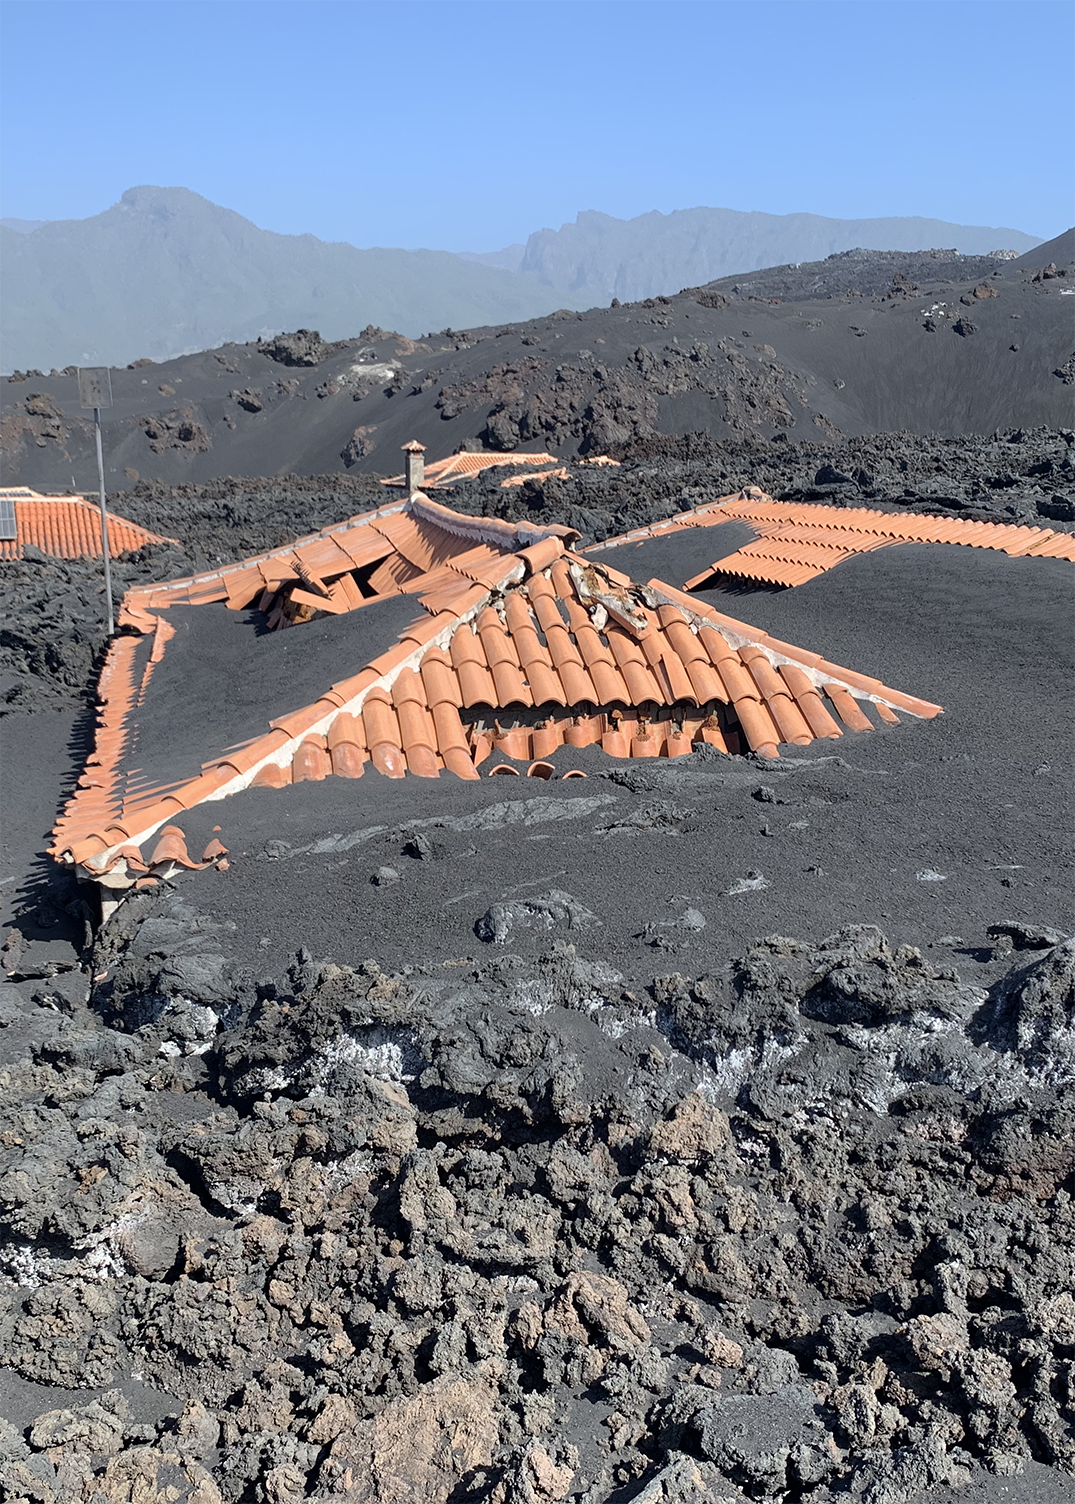
\includegraphics[width=.8\textwidth]{img/tephra-lava.png}
            
        \end{column}
      \end{columns}
\end{frame}


\begin{frame}[t]{Lava flows}
    \begin{columns}[T]
        \begin{column}{0.5\textwidth}	
            \textbf{Modeling} \\ \vspace*{1em} 
            Hazard maps for lava flow inundation using \alert{Q-LavHA}: 
            \begin{itemize}
                \item Uncertainty related to \alert{DEM} and \alert{vent location}
                \item No \alert{physics}!
            \end{itemize}

            \only<2->{
                \vspace*{2em}
                \textbf{Outputs:} \\ \vspace*{1em} 
                \begin{itemize}
                    \item[$\rightarrow$] Probability maps of flow inundation

                \end{itemize}
            }
        \end{column}
  
        \begin{column}{0.5\textwidth}	
            \only<1>{\centering \vspace*{-1em} 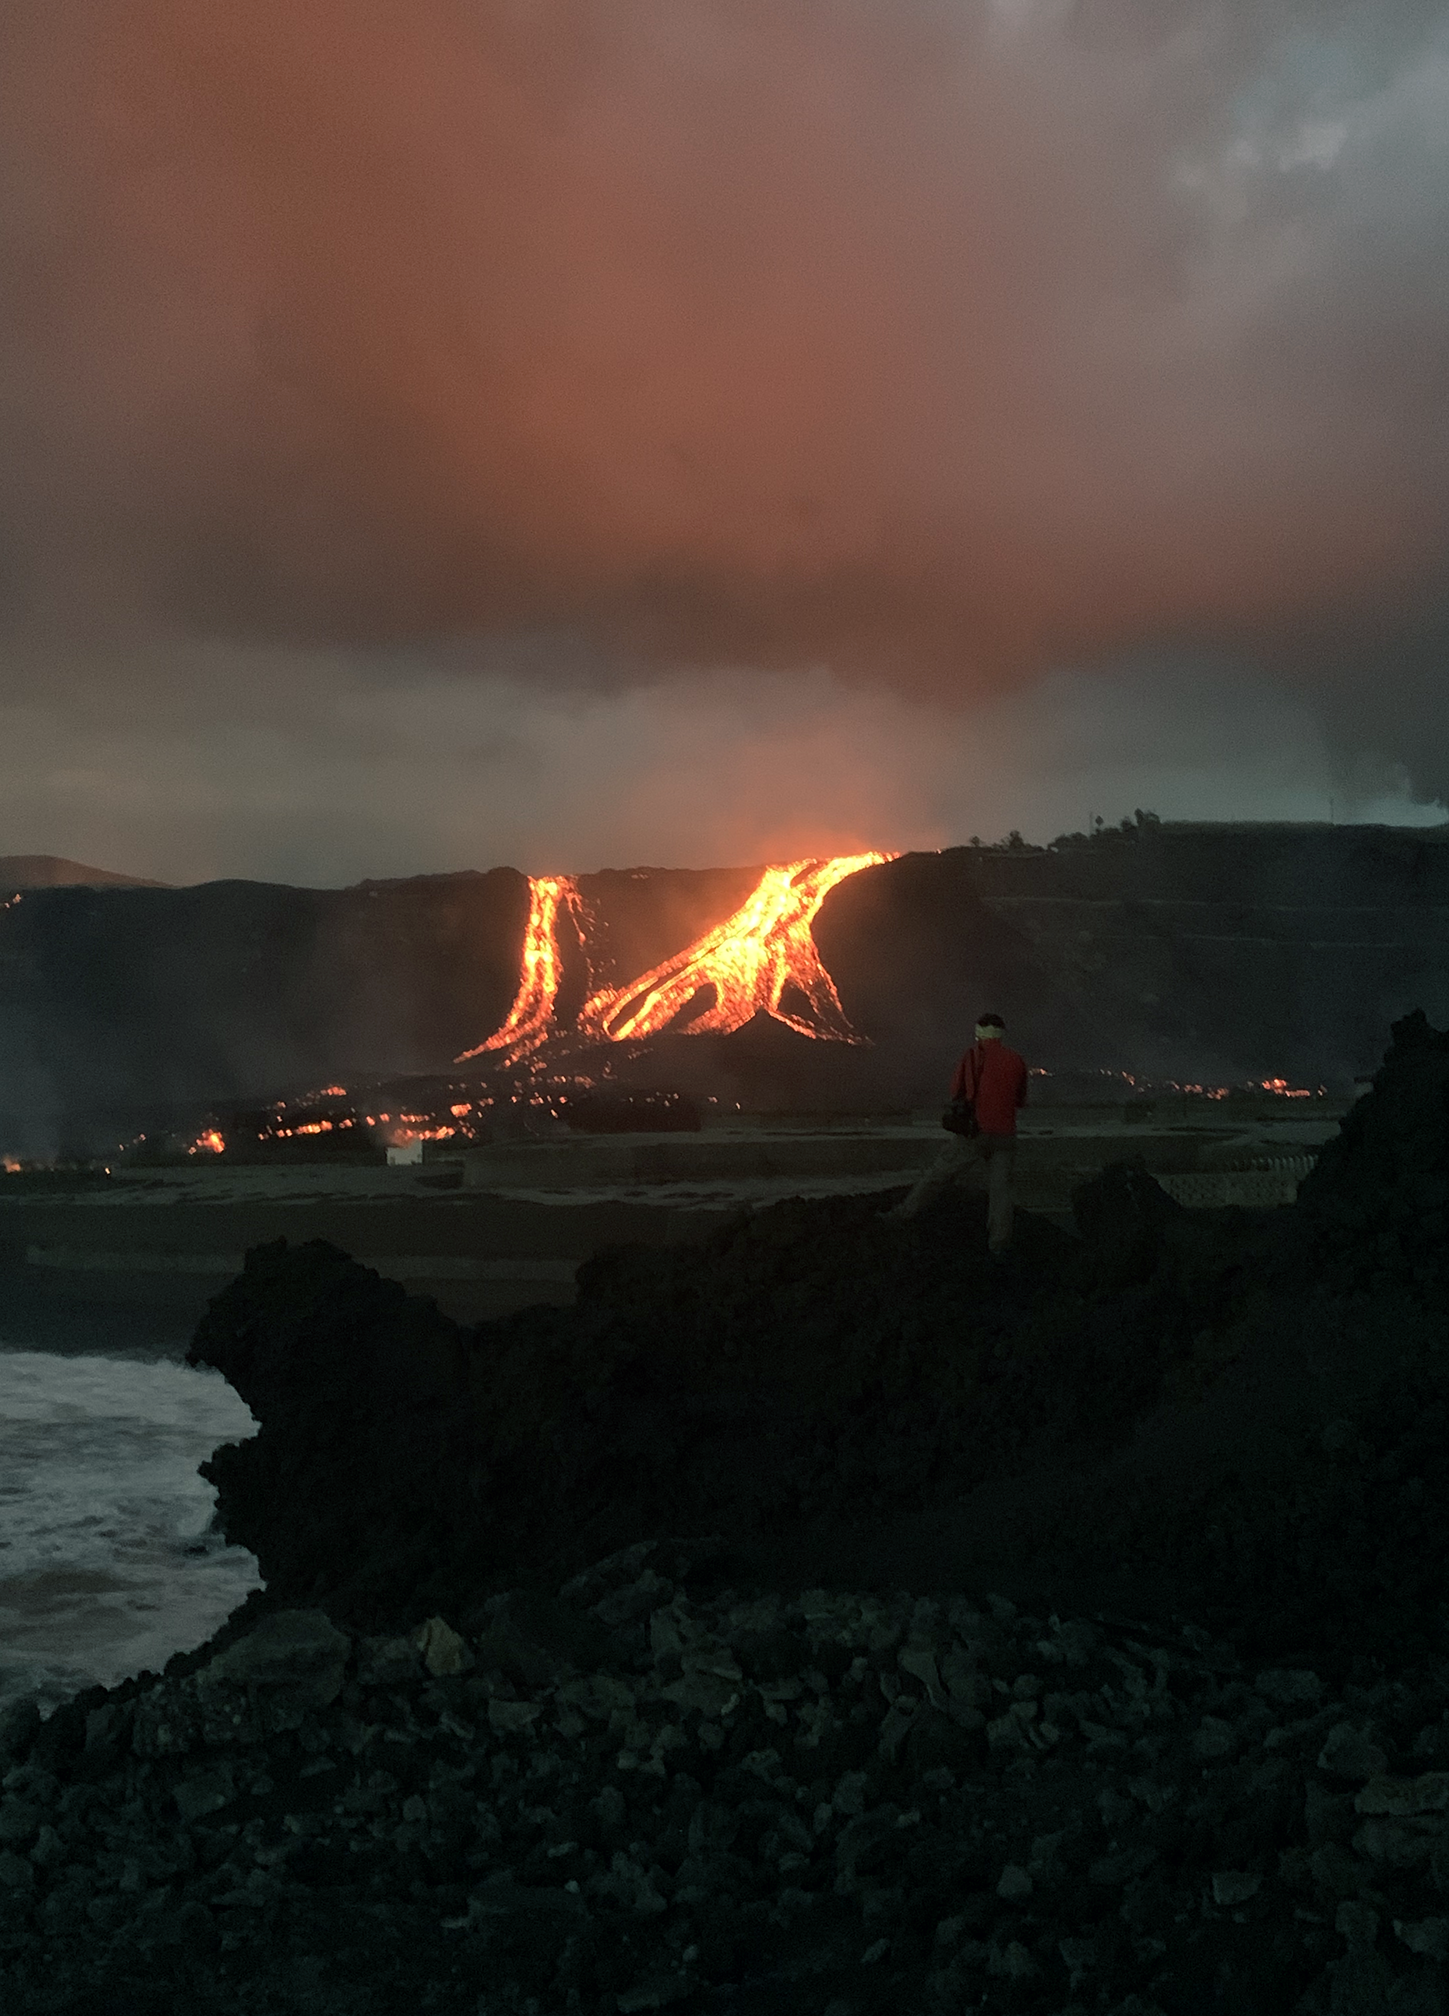
\includegraphics[width=.8\textwidth]{img/lava.png}}
            \only<2>{ \centering \vspace*{-1em} 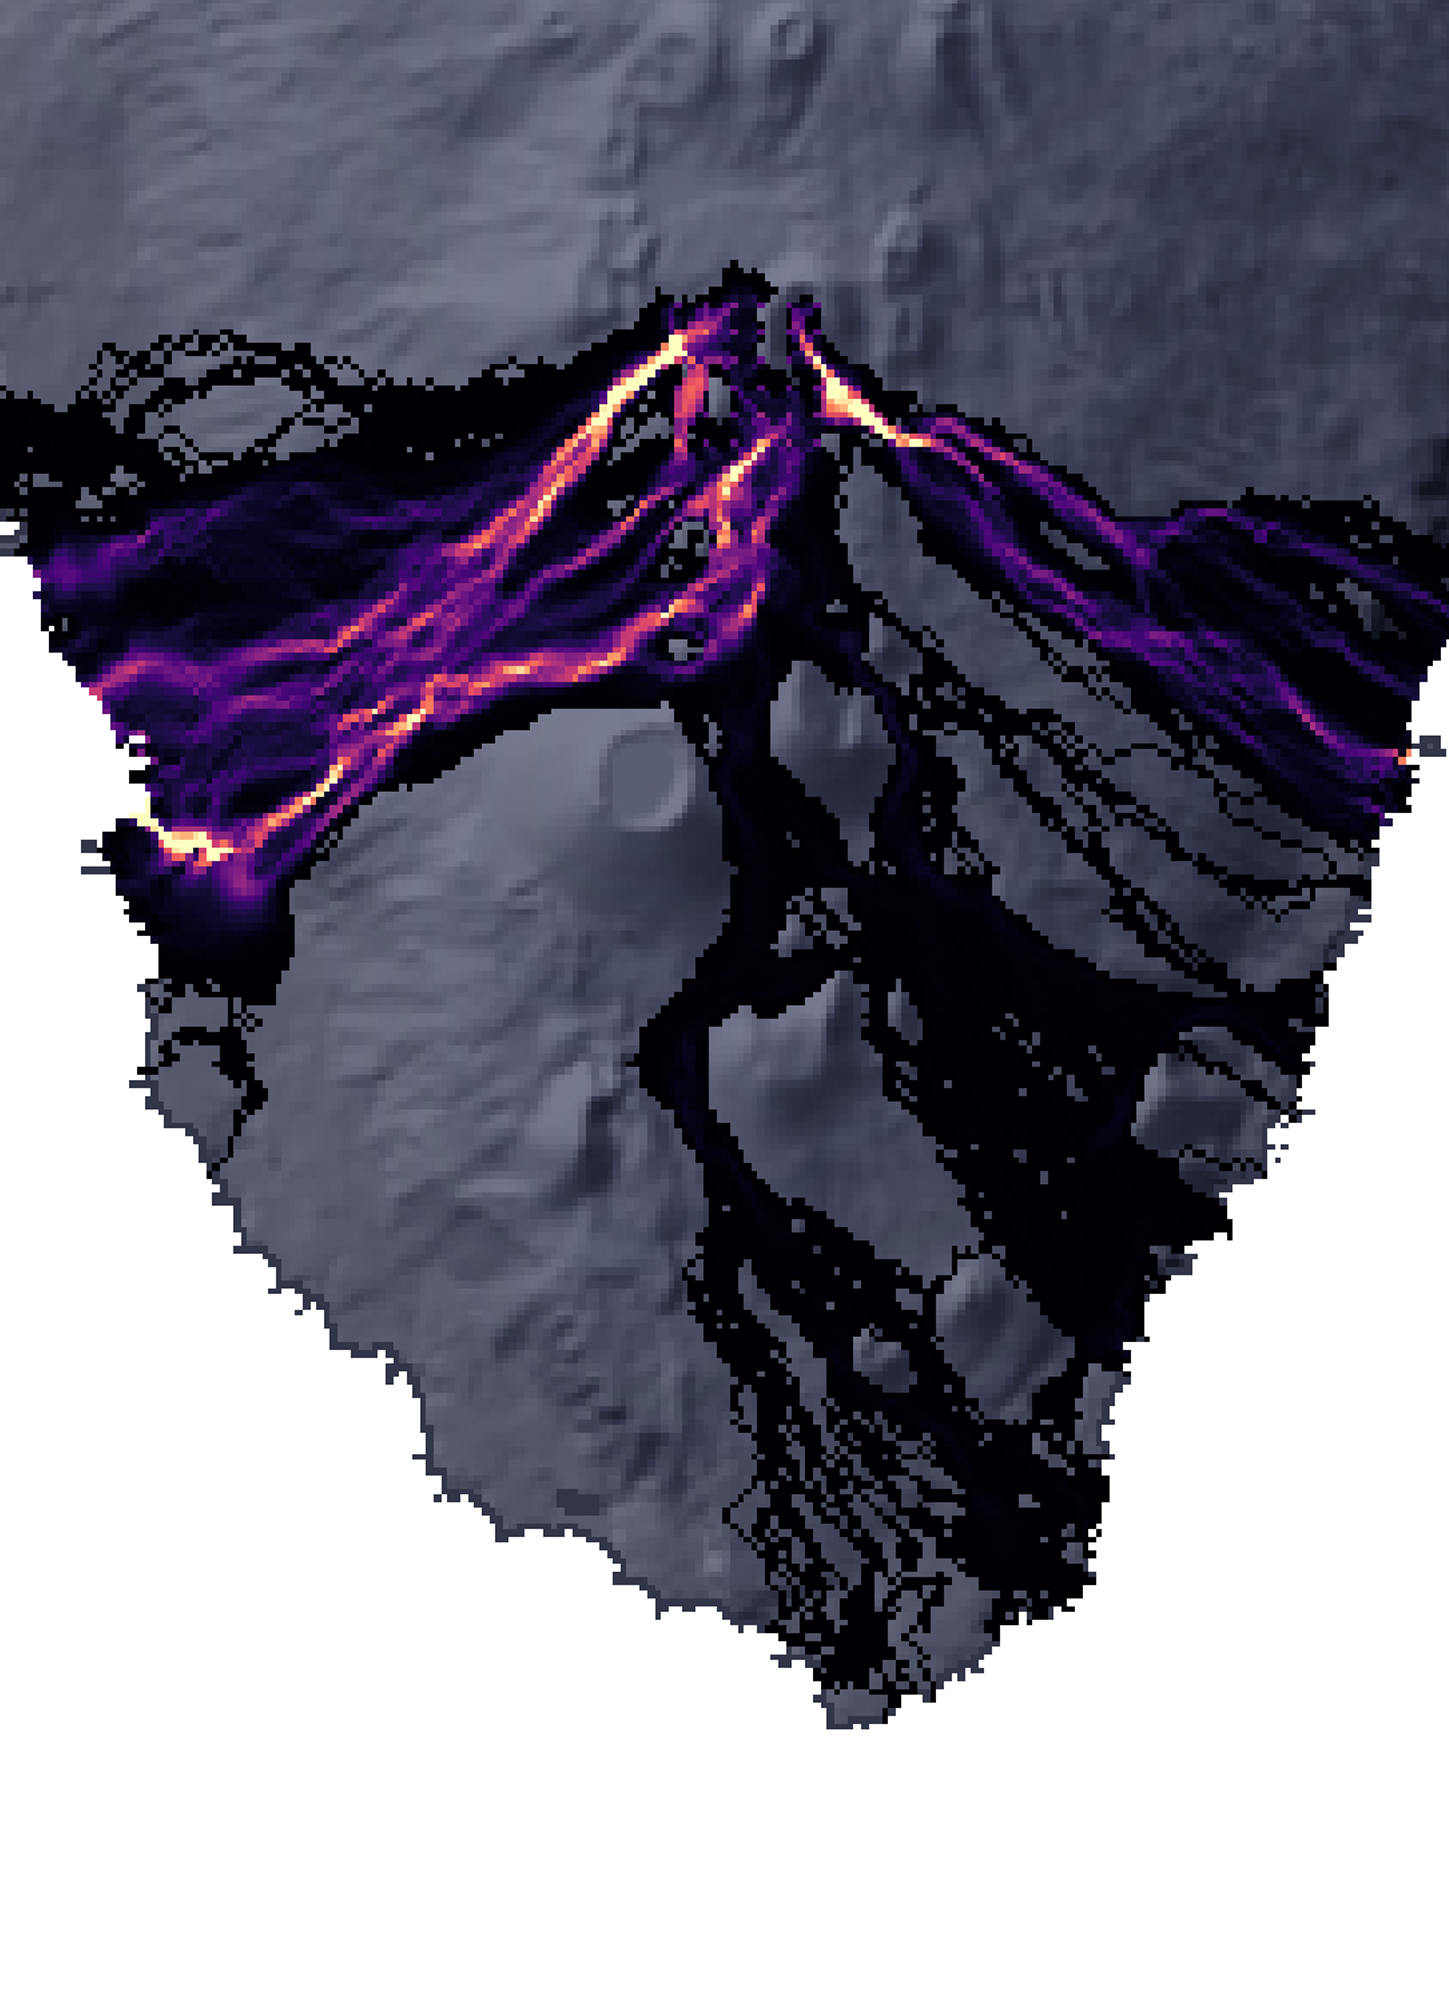
\includegraphics[width=.8\textwidth]{img/hazard_lava.png}}
        \end{column}
      \end{columns}
\end{frame}

\begin{frame}[t]{Tephra fallout}
    \begin{columns}[T]
        \begin{column}{0.5\textwidth}	
            \textbf{Modeling} \\ \vspace*{1em} 
            Hazard maps for tephra accumulation using \alert{TephraProb}: 
            \begin{itemize}
                \item \alert{Sustained} (but \alert{unsteady}!) ash emissions for 3--7 days
                \item Variable \alert{wind conditions}
            \end{itemize}

            \only<2->{
                \vspace*{2em}
                \textbf{Outputs:} \\ \vspace*{1em} 
                \begin{itemize}
                    \item[$\rightarrow$] Probability maps
                    \item[$\rightarrow$] \alert{Probabilistic isomass maps} $\rightarrow$ 25\% and 75\%
                \end{itemize}
            }
        \end{column}
  
        \begin{column}{0.5\textwidth}	
            \only<1>{ \centering \vspace*{-1em} 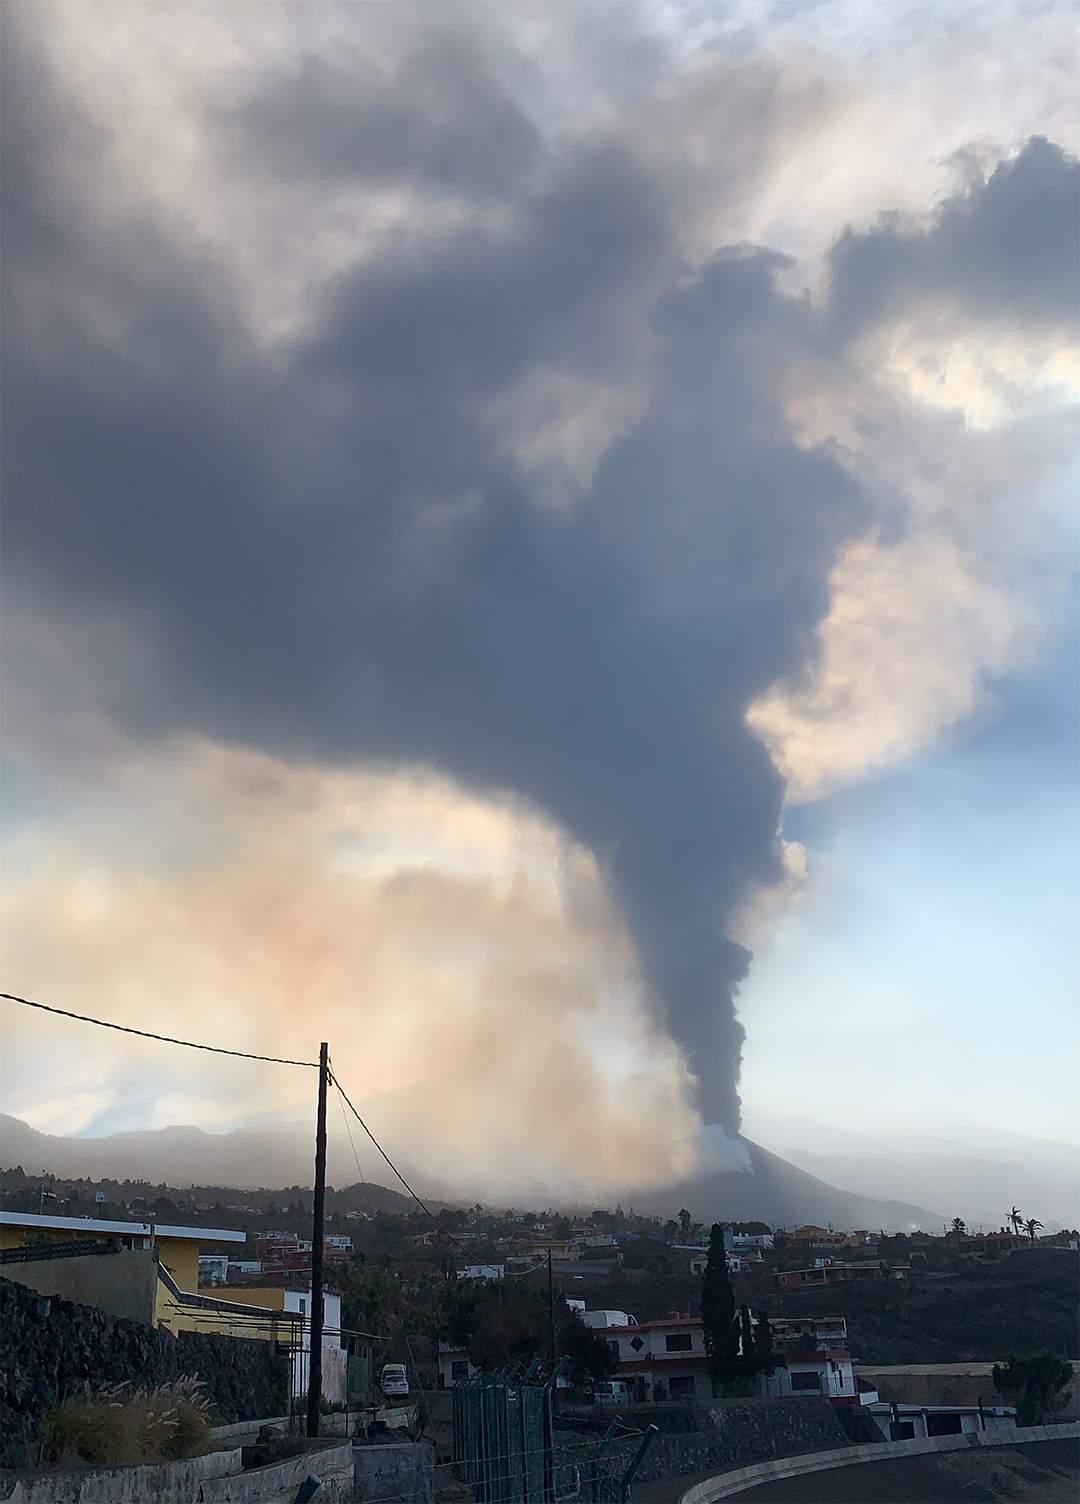
\includegraphics[width=.8\textwidth]{img/tephra-plume.png}}
            \only<2>{ \centering \vspace*{-1em} 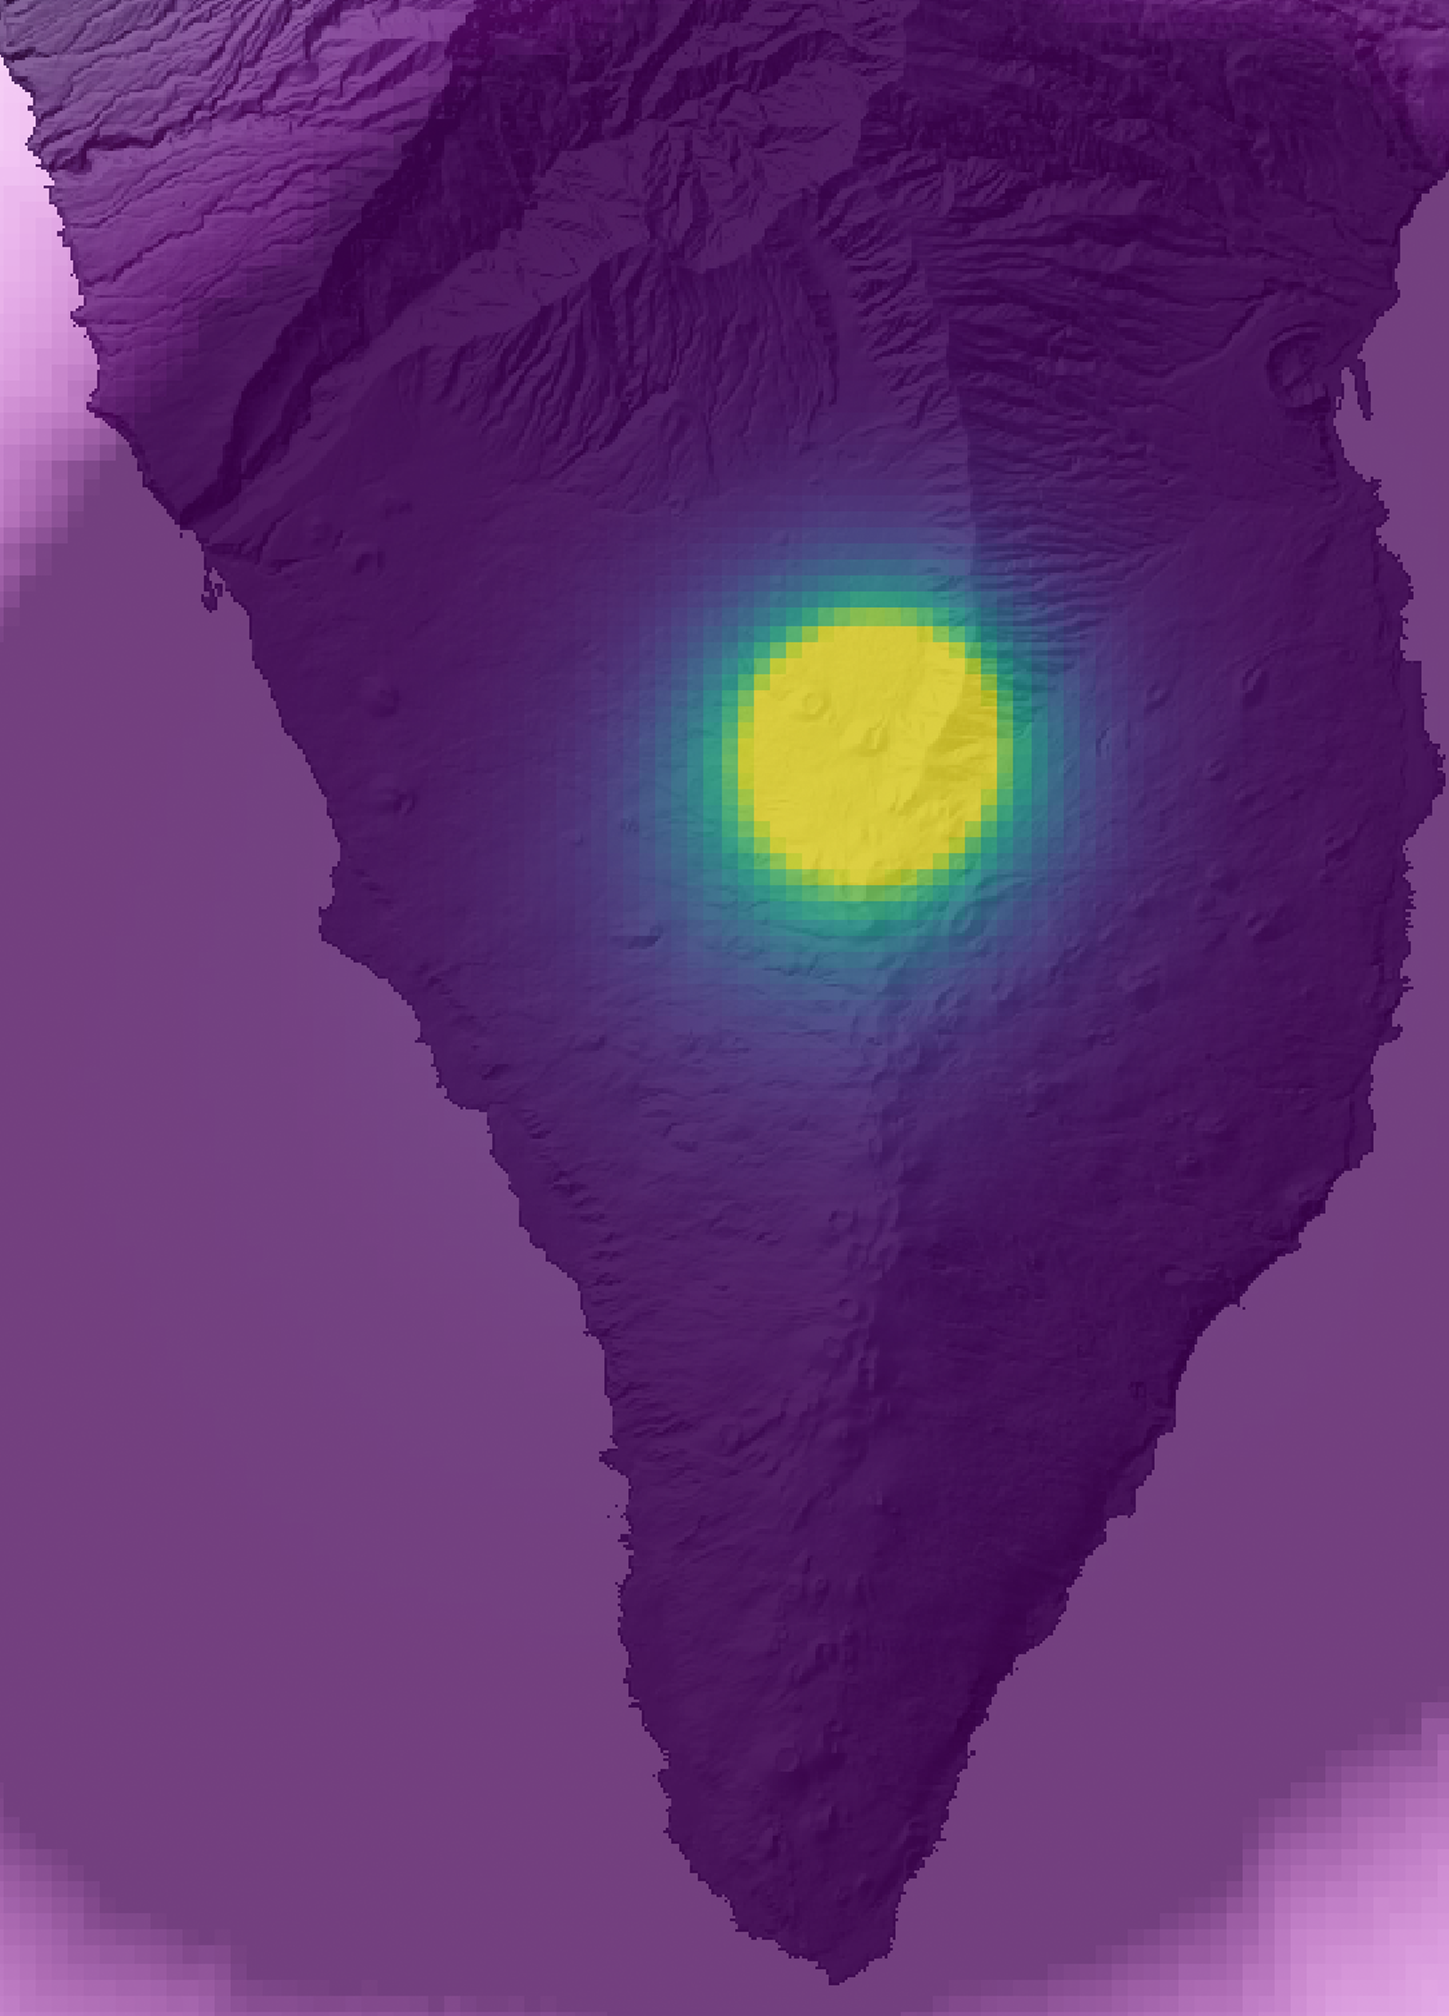
\includegraphics[width=.8\textwidth]{img/hazard_tephra.png}}
        \end{column}
      \end{columns}
\end{frame}

\begin{frame}{Eruption source parameters}
    \only<1>{\centering  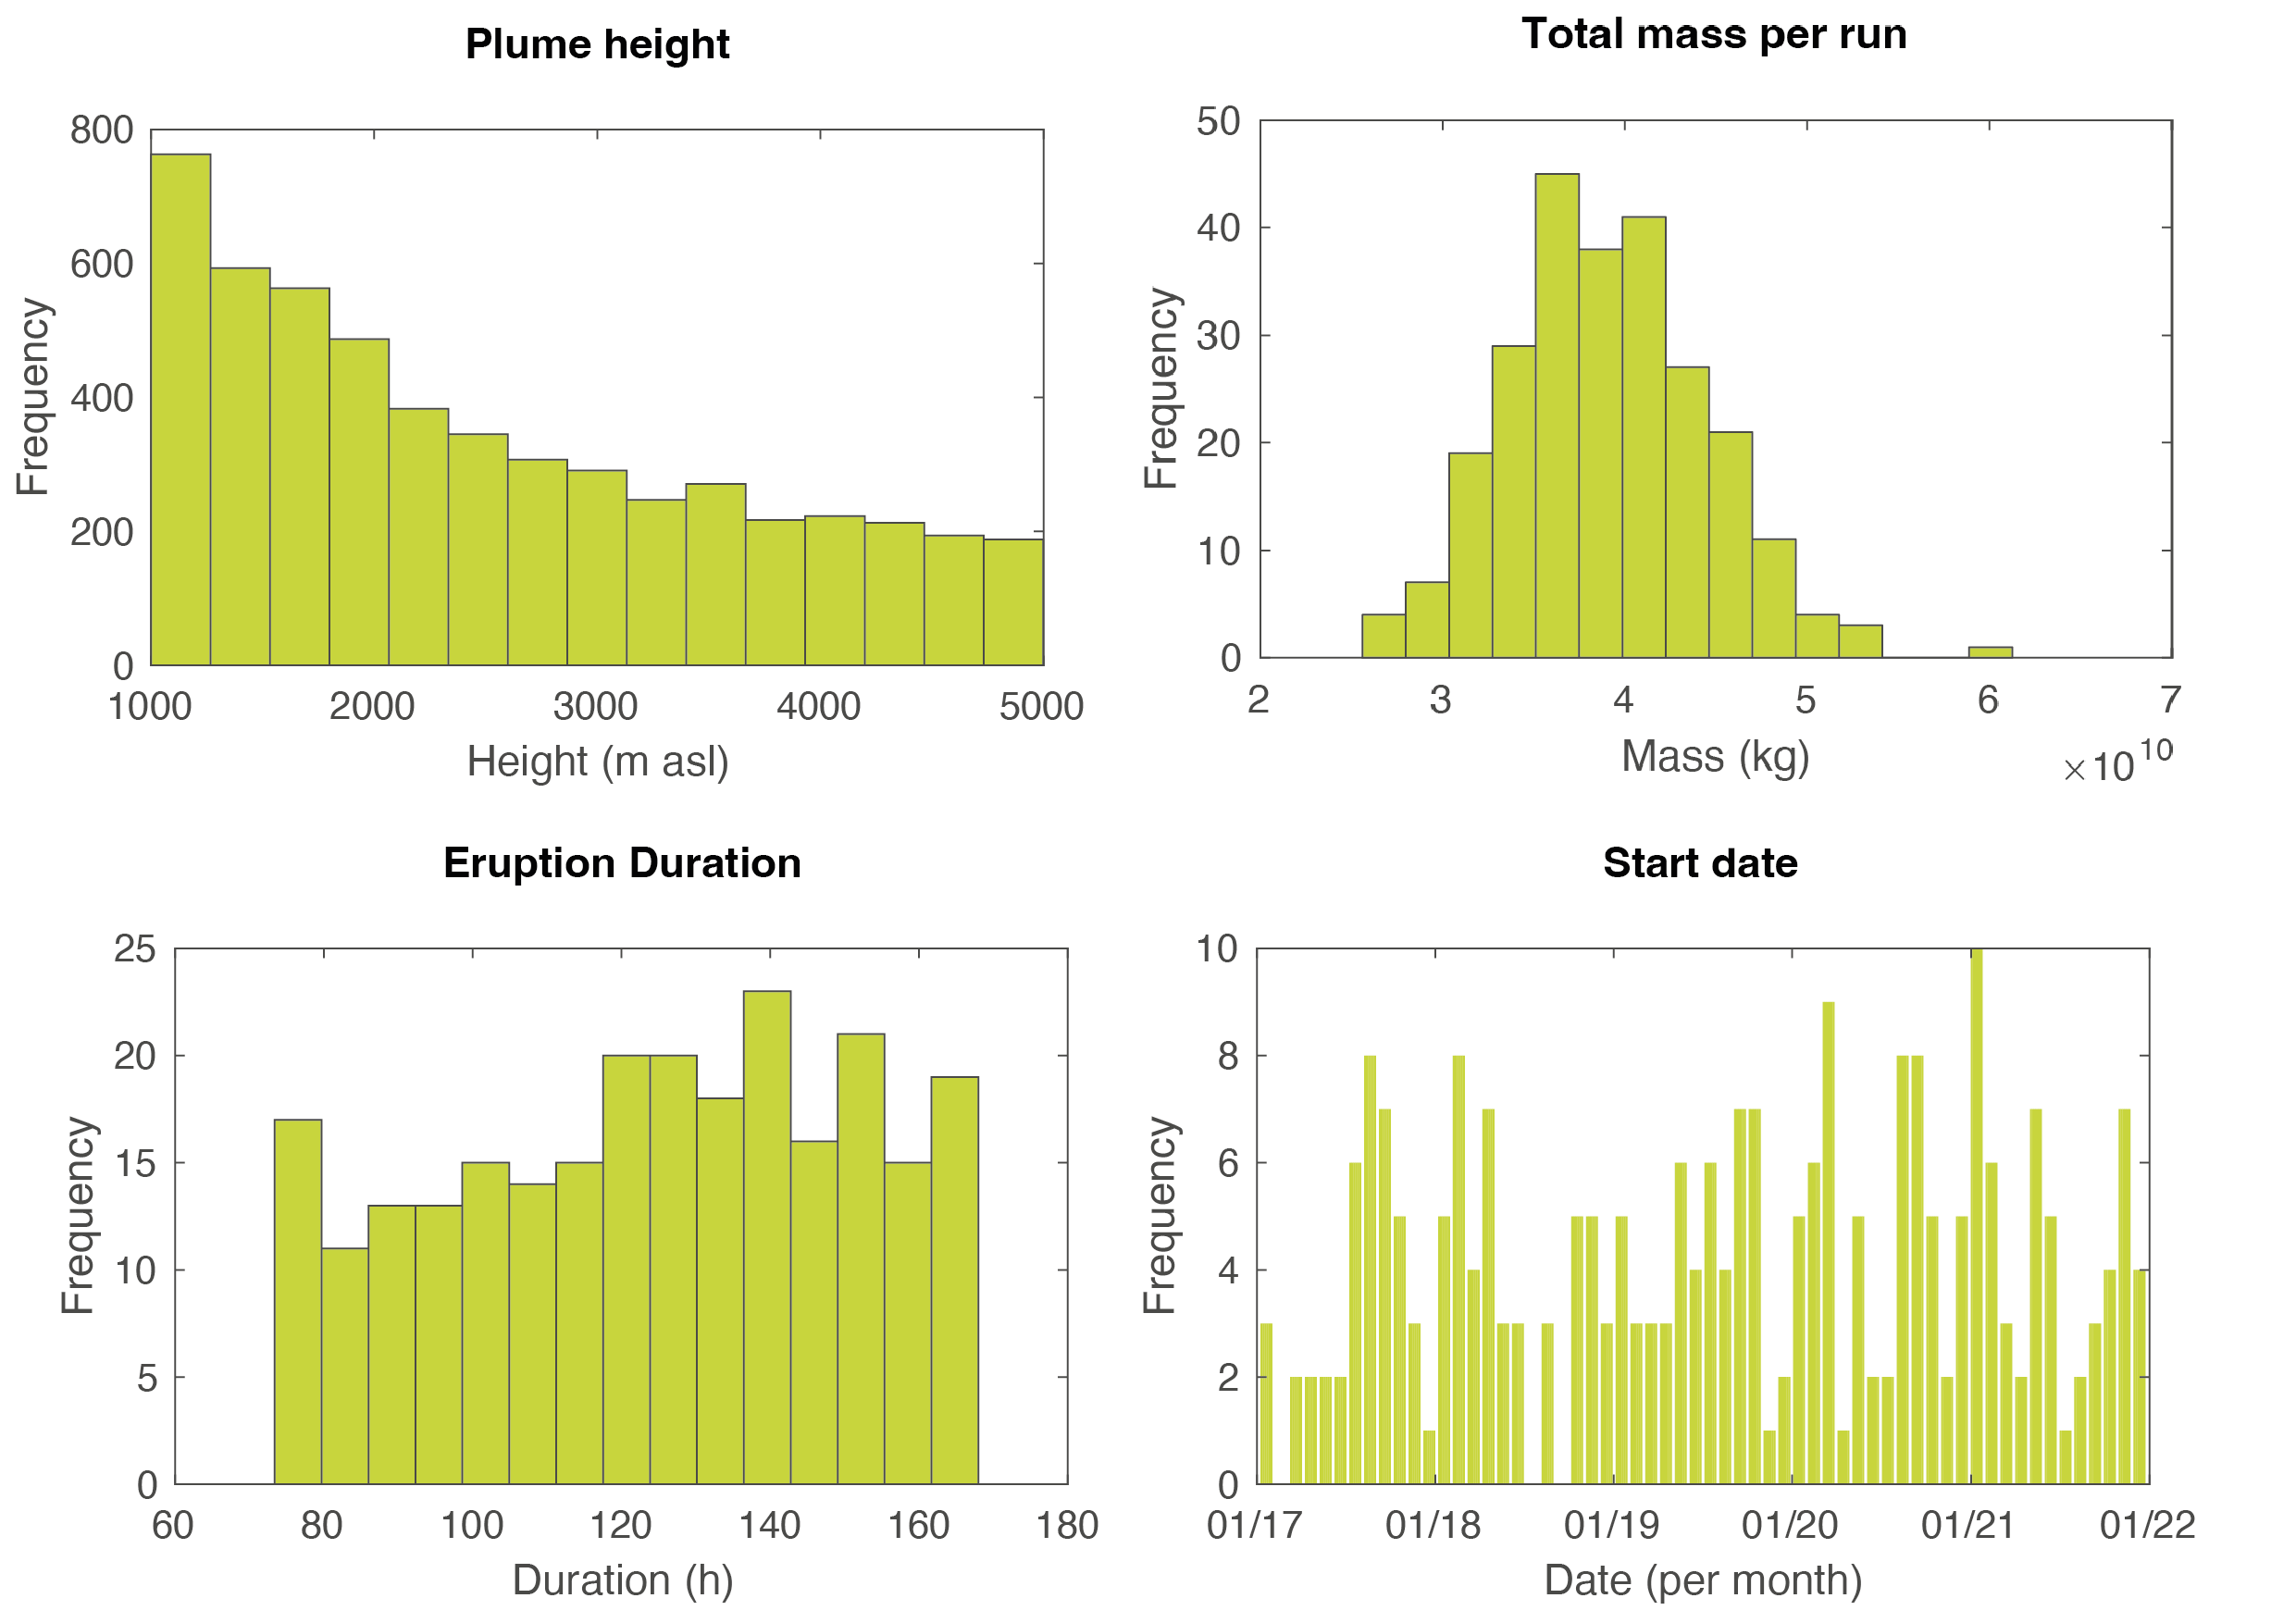
\includegraphics[width=.75\textwidth]{img/esp-grd.png}}
    \only<2>{\centering \hspace*{-2em} 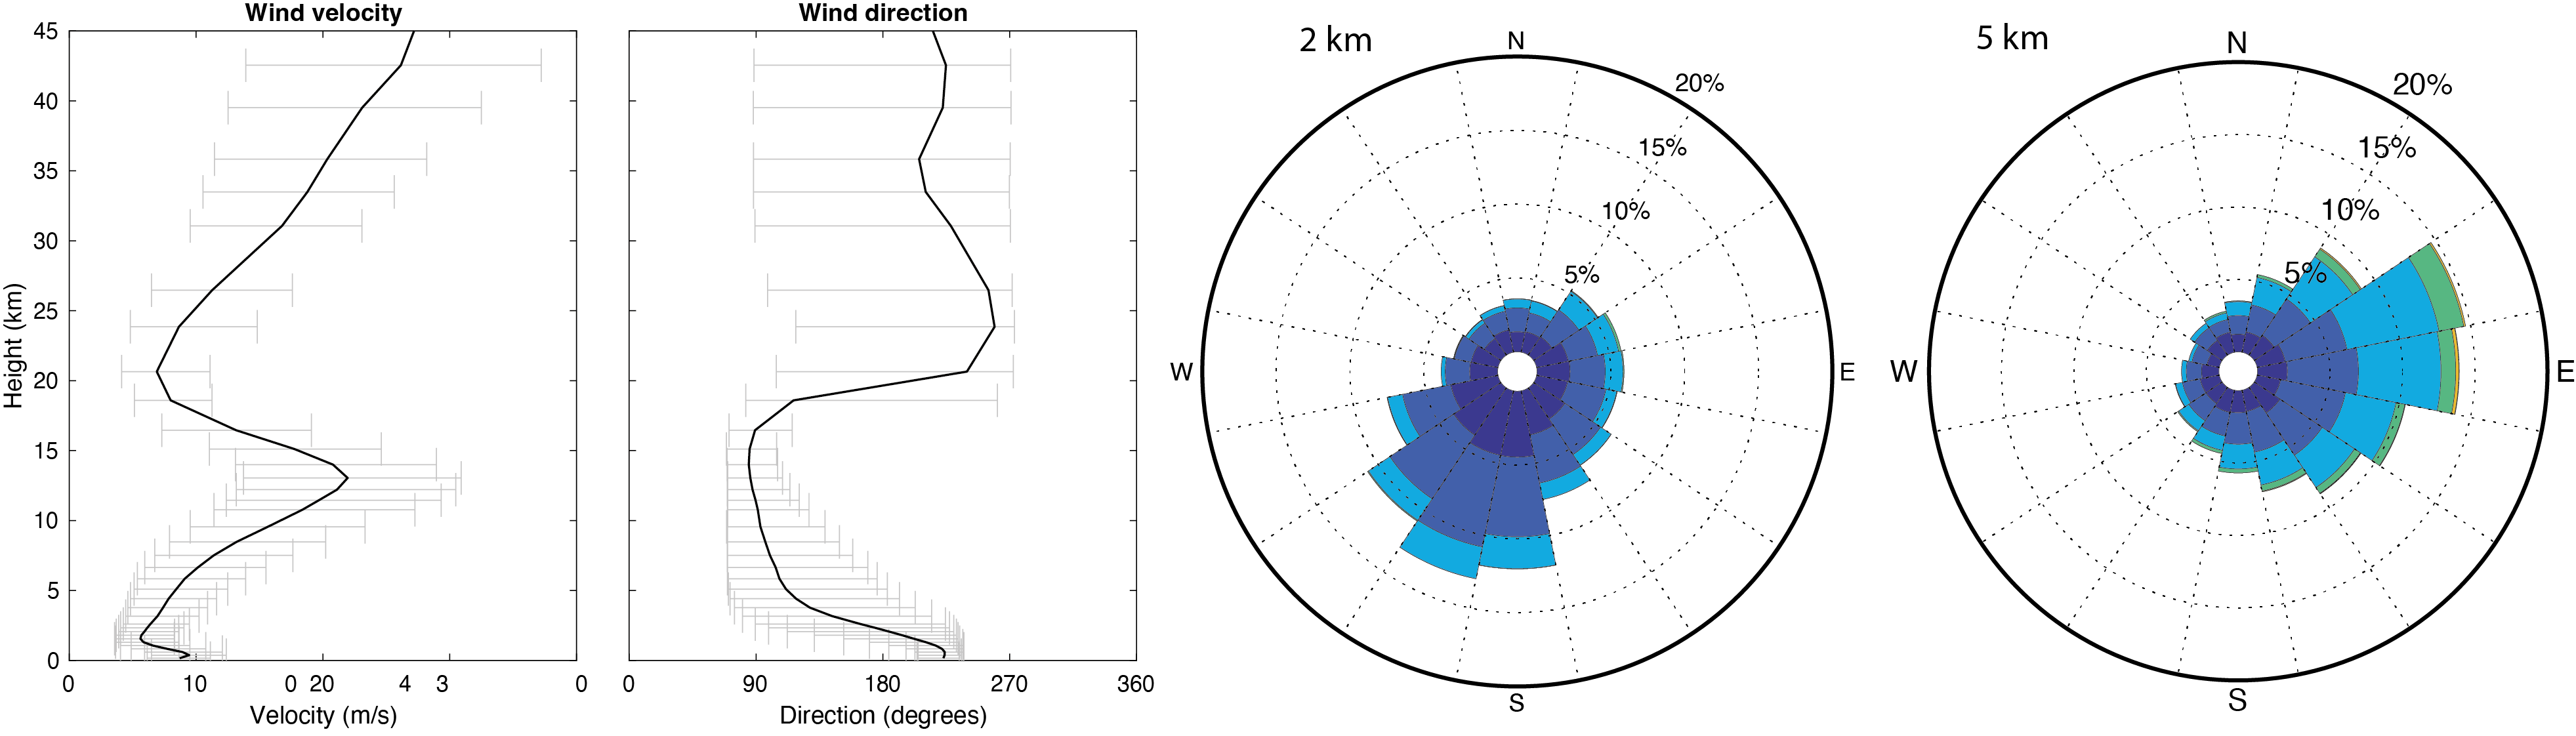
\includegraphics[width=1.1\textwidth]{img/wind.png}}
\end{frame}

\begin{frame}[standout]
  The \alert{exercise}!
\end{frame}


\begin{frame}[t]{Exercise}
\begin{columns}[T]
    \begin{column}{0.5\textwidth}
        \alert<1>{\textbf{Aim:}} Produce a \alert{poster} presenting the hazard assessment for your group	 \\ \vspace*{1em} 
        \only<2->{
            \alert<2>{\textbf{Tephra fallout:} }
            \begin{itemize}
                \item Probabilistic isomass map for a \alert{25\%} probability
                \item Contour the \alert{1}, \alert{10}, \alert{100} and \alert{300} $kg/m^2$ isomass lines
                \item Add any information you might find relevant!
            \end{itemize}
        }
        \only<3->{
            \alert<3>{\textbf{Lava flows:} }
            \begin{itemize}
                \item Highlight \alert{inundation probability}
                \item Be \alert{creative}!
            \end{itemize}
        }
    \end{column}

    \begin{column}{0.5\textwidth}	
        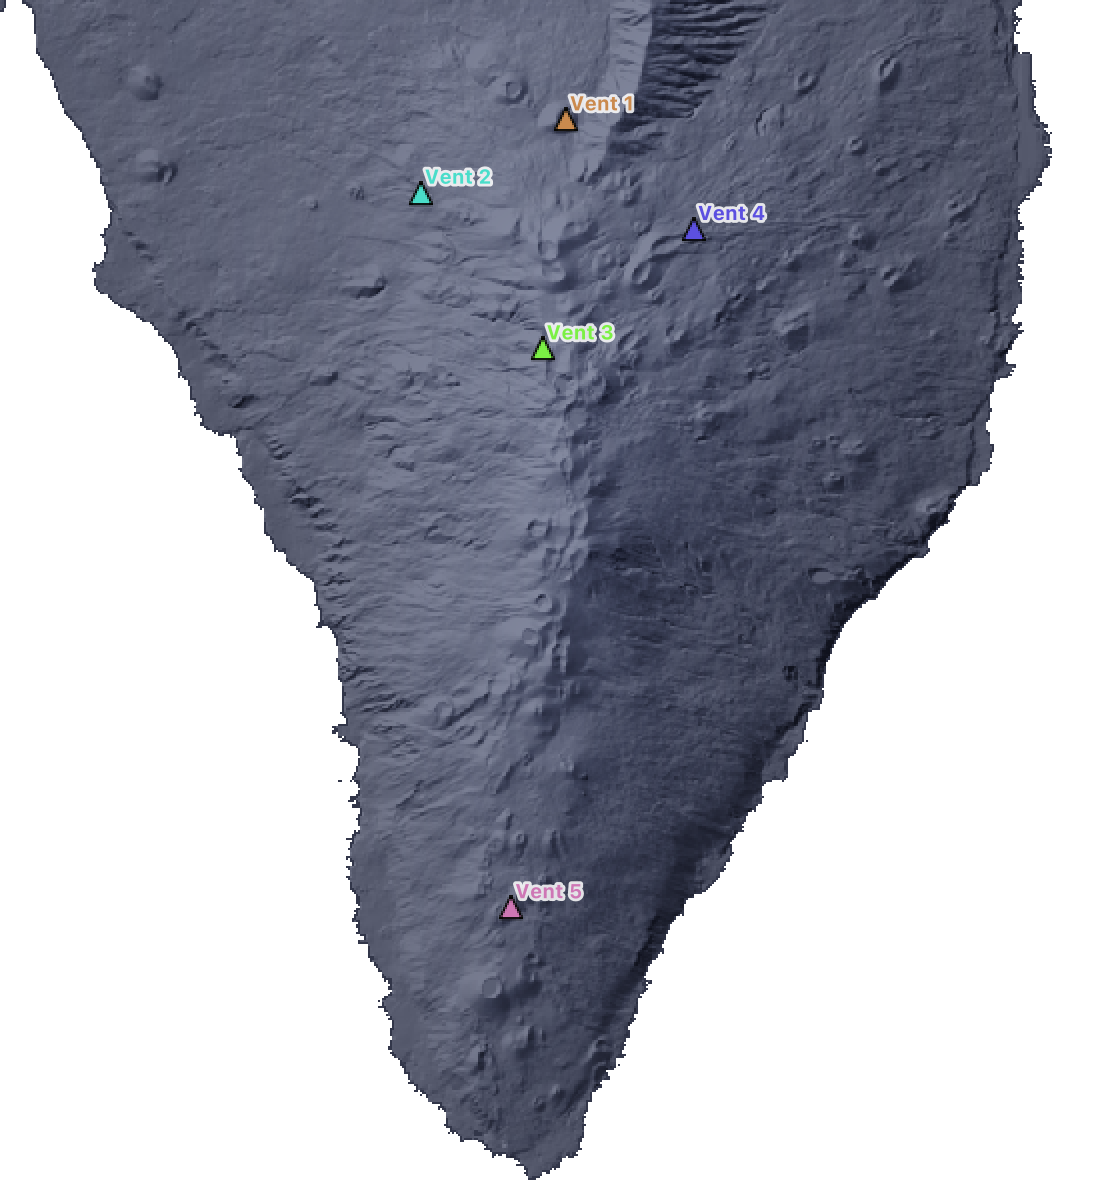
\includegraphics[width=1\textwidth]{img/groups2.png}
    \end{column}
  \end{columns}
\end{frame}

\begin{frame}{Exercise}
    \centering \textbf{Notes:} \\ \vspace*{2em}

    $\rightarrow$ Data on the \alert{USB stick} \\ \vspace*{1em}
    $\rightarrow$ Produce hazard maps on \alert{transparent} paper \\ \vspace*{1em}
    $\rightarrow$ Use \alert{one sheet} per hazard \\ \vspace*{1em}
    $\rightarrow$ \alert{Presentation}: 10 min presentation + 5 min questions  \\ \vspace*{1em}
\end{frame}

    
\begin{frame}{Remember!}
    
\includegraphics[width=\textwidth]{Fig/workflow1.png}
\end{frame}
 

\begin{frame}{Groups}
    \centering
    \begin{table}[htbp]
        \begin{tabular}{m{6em} m{6em} m{6em} m{6em} m{6em} }
            \hline
        \textbf{\alert{Group 1}}  & \textbf{\alert{Group 2}}  & \textbf{\alert{Group 3}}  & \textbf{\alert{Group 4}}  & \textbf{\alert{Group 5}}  \\ \hline
        Fernanda                  & Camille                   & Monique                   & Million                   & Anabella                  \\
        Mattias                   & Giorgi                    & Angie                     & Ana Maria                 & Jonas                     \\
        Florent                   & Amin                      & Karen                     & Génio                     & Nicolas                   \\
        Salome                    & Douglas                   & David                     & Sylvain                   & John                      \\
        Elias                     & Mario                     & Delair                    & Elise                     &                           \\
        \hline
        \end{tabular}%
    \end{table}%
  
  \end{frame}
  
  

\begin{frame}{Questions}
    \textbf{Group 1}: Although the models you have used do not account for time, discuss and contrast the \alert{spatio-temporal evolution} of the selected hazards in the context of a \alert{long-lasting eruption}.

    \textbf{Group 2}: Which \alert{hazard intensity metrics} are used for the selected hazards? Discuss and contrast the different hazard outputs that can be compiled for both hazards.

    \textbf{Group 3}: We only focus here on the hazard associated with tephra accumulation and lava flow inundation, but what other \alert{primary hazards} could occur? 

    \textbf{Group 4}: What \alert{secondary hazards} could occur in association with the selected primary hazards? How could they evolve with time?

    \textbf{Group 5}: What \alert{parameters} affect the selected hazards? Discuss the \alert{objectives} and \alert{pros and cons} of probabilistic versus deterministic approaches.

\end{frame}

\begin{frame}[standout]
    Good luck!
\end{frame}
  

% \begin{frame}{Course's objectives \& schedule}
%   \only<1>{ 
\includegraphics[width=\textwidth]{Fig/workflow1.png} } 
%   \only<2>{

%     \begin{columns}[T]
%       \begin{column}{0.5\textwidth}	
%         \textbf{Day 1: \alert{Lava flow}}        
%           \begin{enumerate}
%             \item Lava flow modeling using several approaches
%             \item Introduction to probabilistic hazard assessment
%             \item Hazard assessment of lava flows
%           \end{enumerate}
%       \end{column}

%       \begin{column}{0.5\textwidth}	
%         \textbf{Day 2: \alert{Tephra fallout}}        
%           \begin{enumerate}
%             \item Introduction to tephra fallouts and ESP
%             \item Deeper into probabilistic hazard assessment
%             \item Probabilistic hazard assessment for tephra fallout
%           \end{enumerate}
%       \end{column}
%     \end{columns}

    
%   } 
% \end{frame}

% \begin{frame}{Some admin}
%   \scriptsize
%   \begin{table}[htbp]
%     \centering
%       \begin{tabular}{llllr}
%       \textbf{\alert{Vent 1}} & \textbf{\alert{Vent 2}} & \textbf{\alert{Vent 3}} & \textbf{\alert{Vent 4}} & \textbf{\alert{Vent 5}} \\ 
%       Fernanda Naranjo Hidalgo & Camille Pastore & Monique Johnson & Million Mengesha & \multicolumn{1}{l}{Anabella Fantozzi} \\
%       Mattias Coullie & John Gallego Montoya & Angie Ramirez Huerta & Ana Maria Perez Hincapie & \multicolumn{1}{l}{Jonas Schranz} \\
%       Florent Keller & Karen Nicollet & Elise Cerutti & Génio Lay Da Silva & \multicolumn{1}{l}{Nicolas Serrano} \\
%       Salome Gogoladze & Douglas Stumpp & David Gutierrez Rivera & Sylvain Köhli & \multicolumn{1}{l}{Amin Abutaleb} \\
%       Elias Garcia Urquia & Mario Cifuentes Jacobs & Delair Ndibi Etoundi & Giorgi Merebashvili &  \\
%       \end{tabular}%
%     \label{tab:addlabel}%
%   \end{table}%
%   \vspace*{2em}
%   \normalsize
%     \centering Theory + lab $\rightarrow$ \alert{Part of the grade!} $\rightarrow$ See question sheet on Moodle
  
% \end{frame}

% % \begin{frame}[standout]
% %   Today: \alert{Lava flows}
% % \end{frame}

% \section{Today: \alert{Lava flows}}

% \begin{frame}{Lava flows}
%   \only<1>{ \centering \includegraphics[width=1\textwidth]{img/lava_flow.png} \\ \vspace*{1em}
%     Lava channel $\rightarrow$ A'a $\rightarrow$ Pahoehe \\  
%   }
% \end{frame}

% % - Lava flows -> infrastructures
% % - Hawaii, DRC, La Palma
% % - Slow moving, not lethal, but
% % - Long lasting crises, high uncertainties
% % - Complex phenomenon, can extend 10th of km from the source 
% % - Emergency management is complex, requires proper channels of communication between scientific institutions, decision makers, stakeholders

% \begin{frame}{Pahoa crisis, Hawaii, 2014}
%   \only<1>{ \centering \includegraphics[width=.55\textwidth]{img/HI.pdf} }
%   \only<2>{ \centering 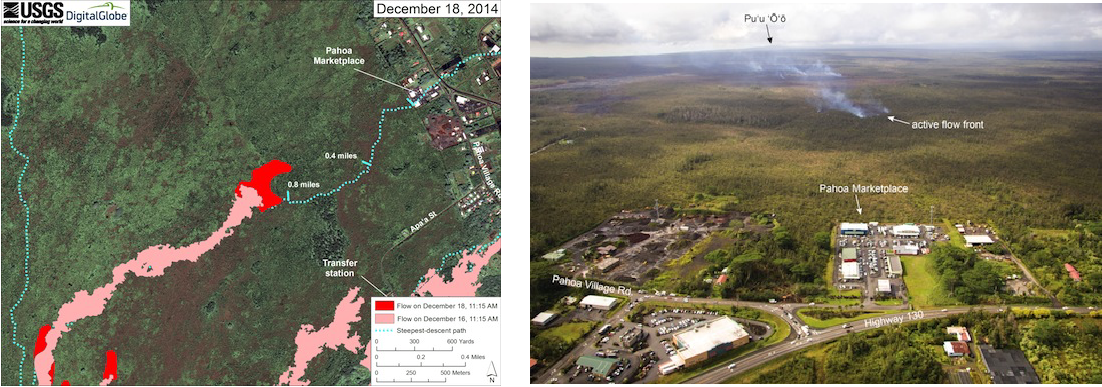
\includegraphics[width=1\textwidth]{img/pahoa.png} }
% \end{frame}

% % - Communication: Puhoho active since the 80's
% % - Repeated impacts on the community

% \section{\alert{Lava flow part I} \\Path of steepest descent}

% \begin{frame}[t]{Path of steepest descent}
%   \begin{columns}[T]
%     \begin{column}{0.5\textwidth}	
%       \only<1>{
%         \centering 
%         \textbf{DEM}: Digital Elevation Models \\
%         $\downarrow$ \\ 
%         \textbf{Hydrological models}  \\ 
%         $\downarrow$ \\ 
%         \texttt{Flow accumulation} $\rightarrow$ \texttt{Stream network} $\rightarrow$ \texttt{Drainage basins}
%       }
%       \only<2>{
%         \textbf{Flow accumulation}
%         \begin{itemize}
%           \item \alert{Cumulative number of upstream pixels that contribute to surface water drainage to any given downstream pixel}
%           \item From any pixel, flow goes in the direction of the \alert{largest} $-\Delta Z$
%           \item Once flow direction is estimated, the algorithm counts \alert{how many upstream pixels} contribute to any given downstream pixel
%         \end{itemize}
%       }
%       \only<3>{
%         \textbf{Stream network}
%         \begin{itemize}
%           \item Applies a threshold of count values $c$ to the \alert{Flow Accumulation} raster to delineate a \textbf{stream}
%           \item If a given pixel has a number of contributing pixels $C$ such as $C \geq c$, then the pixel is assumed to be part of the stream
%           \item \alert{Stream} network is a synonym of \alert{path of steepest descent}
%         \end{itemize}
%       }
%       \only<4>{
%         \textbf{Drainage basins}
%         \begin{itemize}
%           \item Classifies which stream each pixel contributes to. 
%           \item Think of it as a watershed, where ridges act as limits between zone contributing to different streams and valleys accumulate most of the surface flow.
%         \end{itemize}
%       }
%     \end{column}

%     \begin{column}{0.5\textwidth}	
%       \only<1>{
%         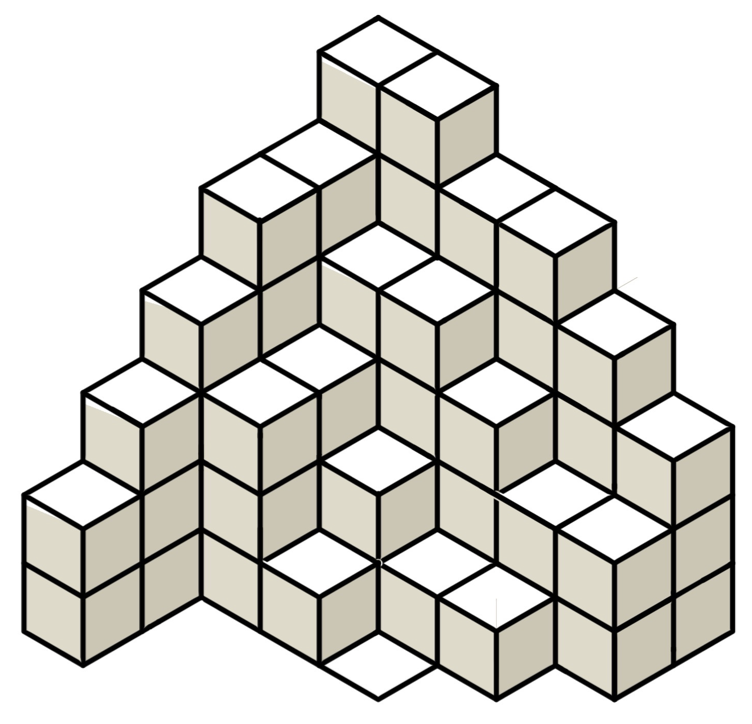
\includegraphics[width=1\textwidth]{../docs/img/hydro/hydro1.png}
%       }
%       \only<2>{
%         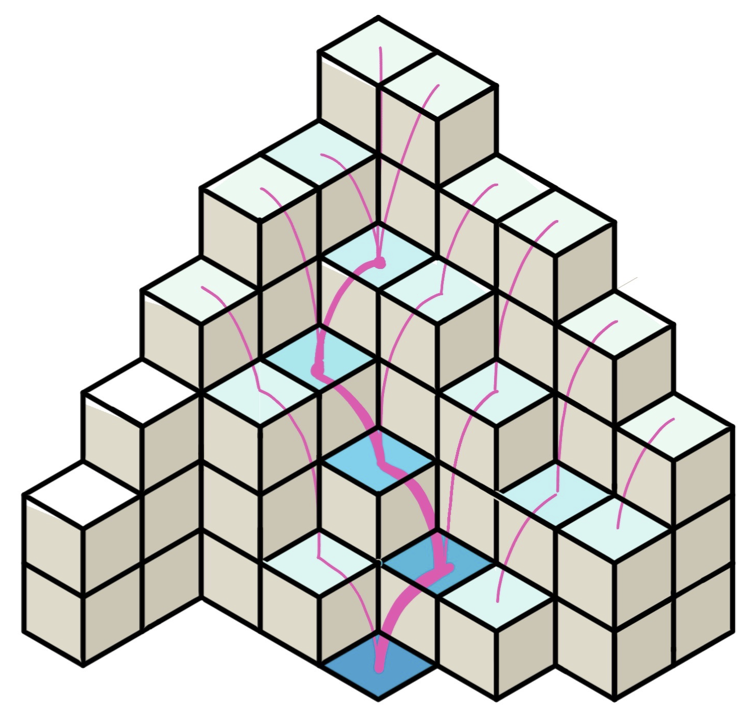
\includegraphics[width=1\textwidth]{../docs/img/hydro/hydro2.png}
%       }
%       \only<3>{
%         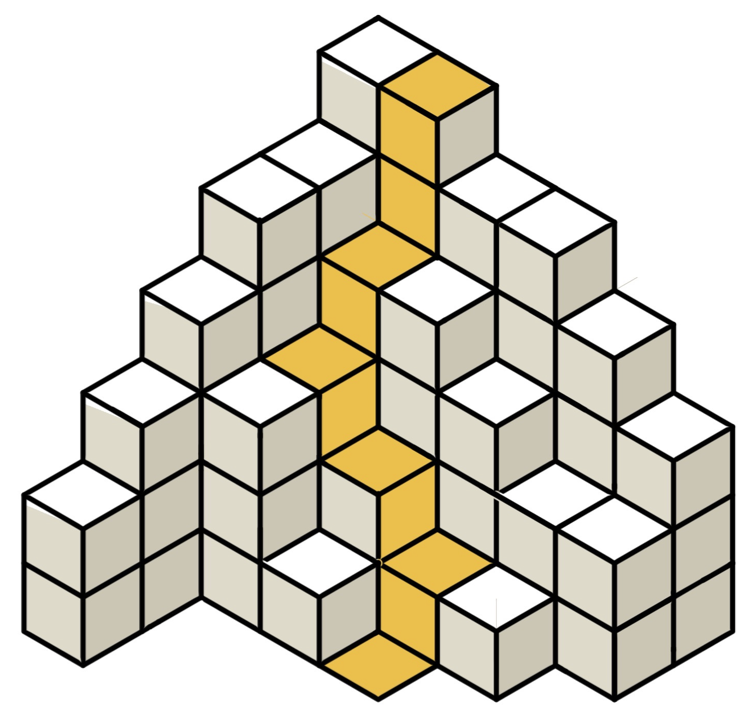
\includegraphics[width=1\textwidth]{../docs/img/hydro/hydro3.png}
%         }
%         \only<4>{
%         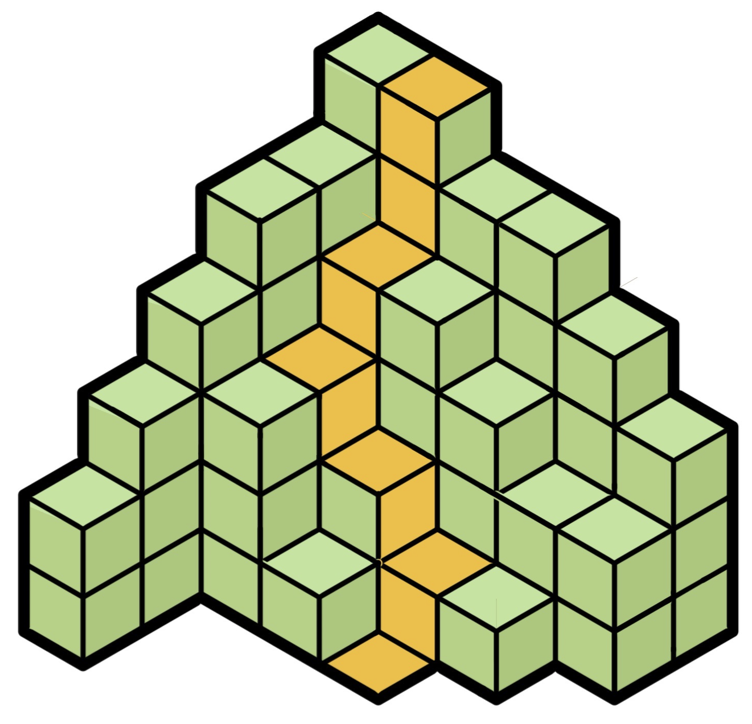
\includegraphics[width=1\textwidth]{../docs/img/hydro/hydro4.png}
%       }
%     \end{column}
%   \end{columns}
% \end{frame}

% \begin{frame}[standout]
%   \alert{Exercise 1:} Path of steepest descent for La Palma \\ \vspace*{1em}
% \end{frame}

% \begin{frame}[t]{Exercise 1: Path of steepest descent for La Palma}
  
%   \only<1-2>{
%     \textbf{Aims:}
%     \begin{itemize}
%       \item Analyse \alert{hydrological properties} of la Palma based on a 25-m DEM 
%       \item Revisit \alert{historical lava flows} based on the geological map
%       \item Get a \alert{critical} perspective on the path of steepest descent approach
%     \end{itemize} 
%   }

%   \only<2>{
%     \textbf{Workflow:}
%     \begin{itemize}
%       \item Go to http://cerg-c.github.io 
%       \item Go through the following exercises:
%       \begin{itemize}
%         \item \alert{Teaching / Setting up QGIS}
%         \item \alert{Teaching / Lava hazard / Introduction}
%         \item \alert{Teaching / Lava hazard / Getting started}
%         \item \alert{Teaching / Lava hazard / Steepest descent}
%       \end{itemize}
%     \end{itemize}
%     }
%   \only<4>{
%     \textbf{Don't forget} to fill up the \alert{questions sheet}!\\
%   }
%   \only<3->{
%     \vspace*{2em}
%     \textbf{Let's get started together}
%     \begin{enumerate}
%       \item Start \alert{QGIS}, change language
%       \item Install \alert{Q-LavHA}
%       \item \alert{Download} and \alert{load} QIS data
%     \end{enumerate}
%   }



%   \end{frame}


% \begin{frame}[standout]
%   How likely are you to recommend the \alert{path of steepest descent} to a friend?\\
%   $\star \star \star \star \star $
% \end{frame}

% \section{\alert{Lava flow part II} \\ Modeling lava flows}

% \begin{frame}{When and why do lava flows?}

%     \begin{columns}[T]
%       \begin{column}{0.65\textwidth}	

%         \only<1-2>{
%           \textbf{Shear stress}\\ \vspace*{.5em}
          
%           The shear stress $\tau$ is the \alert{load stress applied to a fluid} $\rightarrow$ i.e., the force per unit area acting in the direction and parallel to the flow surface:

%           $$ \tau = \rho g h \times sin(\alpha)\ [Pa = Nm^{-2}]  $$
%         }

%         \only<2>{
%           \textbf{Strain rate}\\ \vspace*{.5em}
%           The strain rate $\epsilon$ is the \alert{rate of deformation} when a shear stress is applied $\rightarrow$ i.e., velocity gradient:

%           $$ \epsilon = \frac{dV}{dZ}\ [s^{-1}] $$

%         }

%         \only<3-4>{
%           \textbf{Yield strength}\\ \vspace*{.5em}
          
%           The yield strength $\tau _0$ is the \alert{shear stress} above which deformation begins**:

%           $$\tau_0 = \rho g h_0 \times sin(\alpha)\ [Pa = Nm^{-2          }]$$
%         }

%         \only<4>{

%           \textbf{Viscosity}\\ \vspace*{.5em}

%           The viscosity $\eta$ is the \alert{resistance of fluid} to flow when shear stress is applied:

%           $$\eta = \frac{d\tau}{d\epsilon}\ [Pa\ s = Nm^{-2}          s]$$

%         }

%         \only<5>{
%           \textbf{Summary:}\\ \vspace*{.5em}
%           \begin{itemize}
%             \item Flow occurs when \textbf{driving forces} \alert{exceed} \textbf{resistive forces}
%             \item Response/behaviour of the fluid depends on its \textbf{rheology}
%           \end{itemize}
%         }

%       \end{column}

%       \begin{column}{0.35\textwidth}	
%         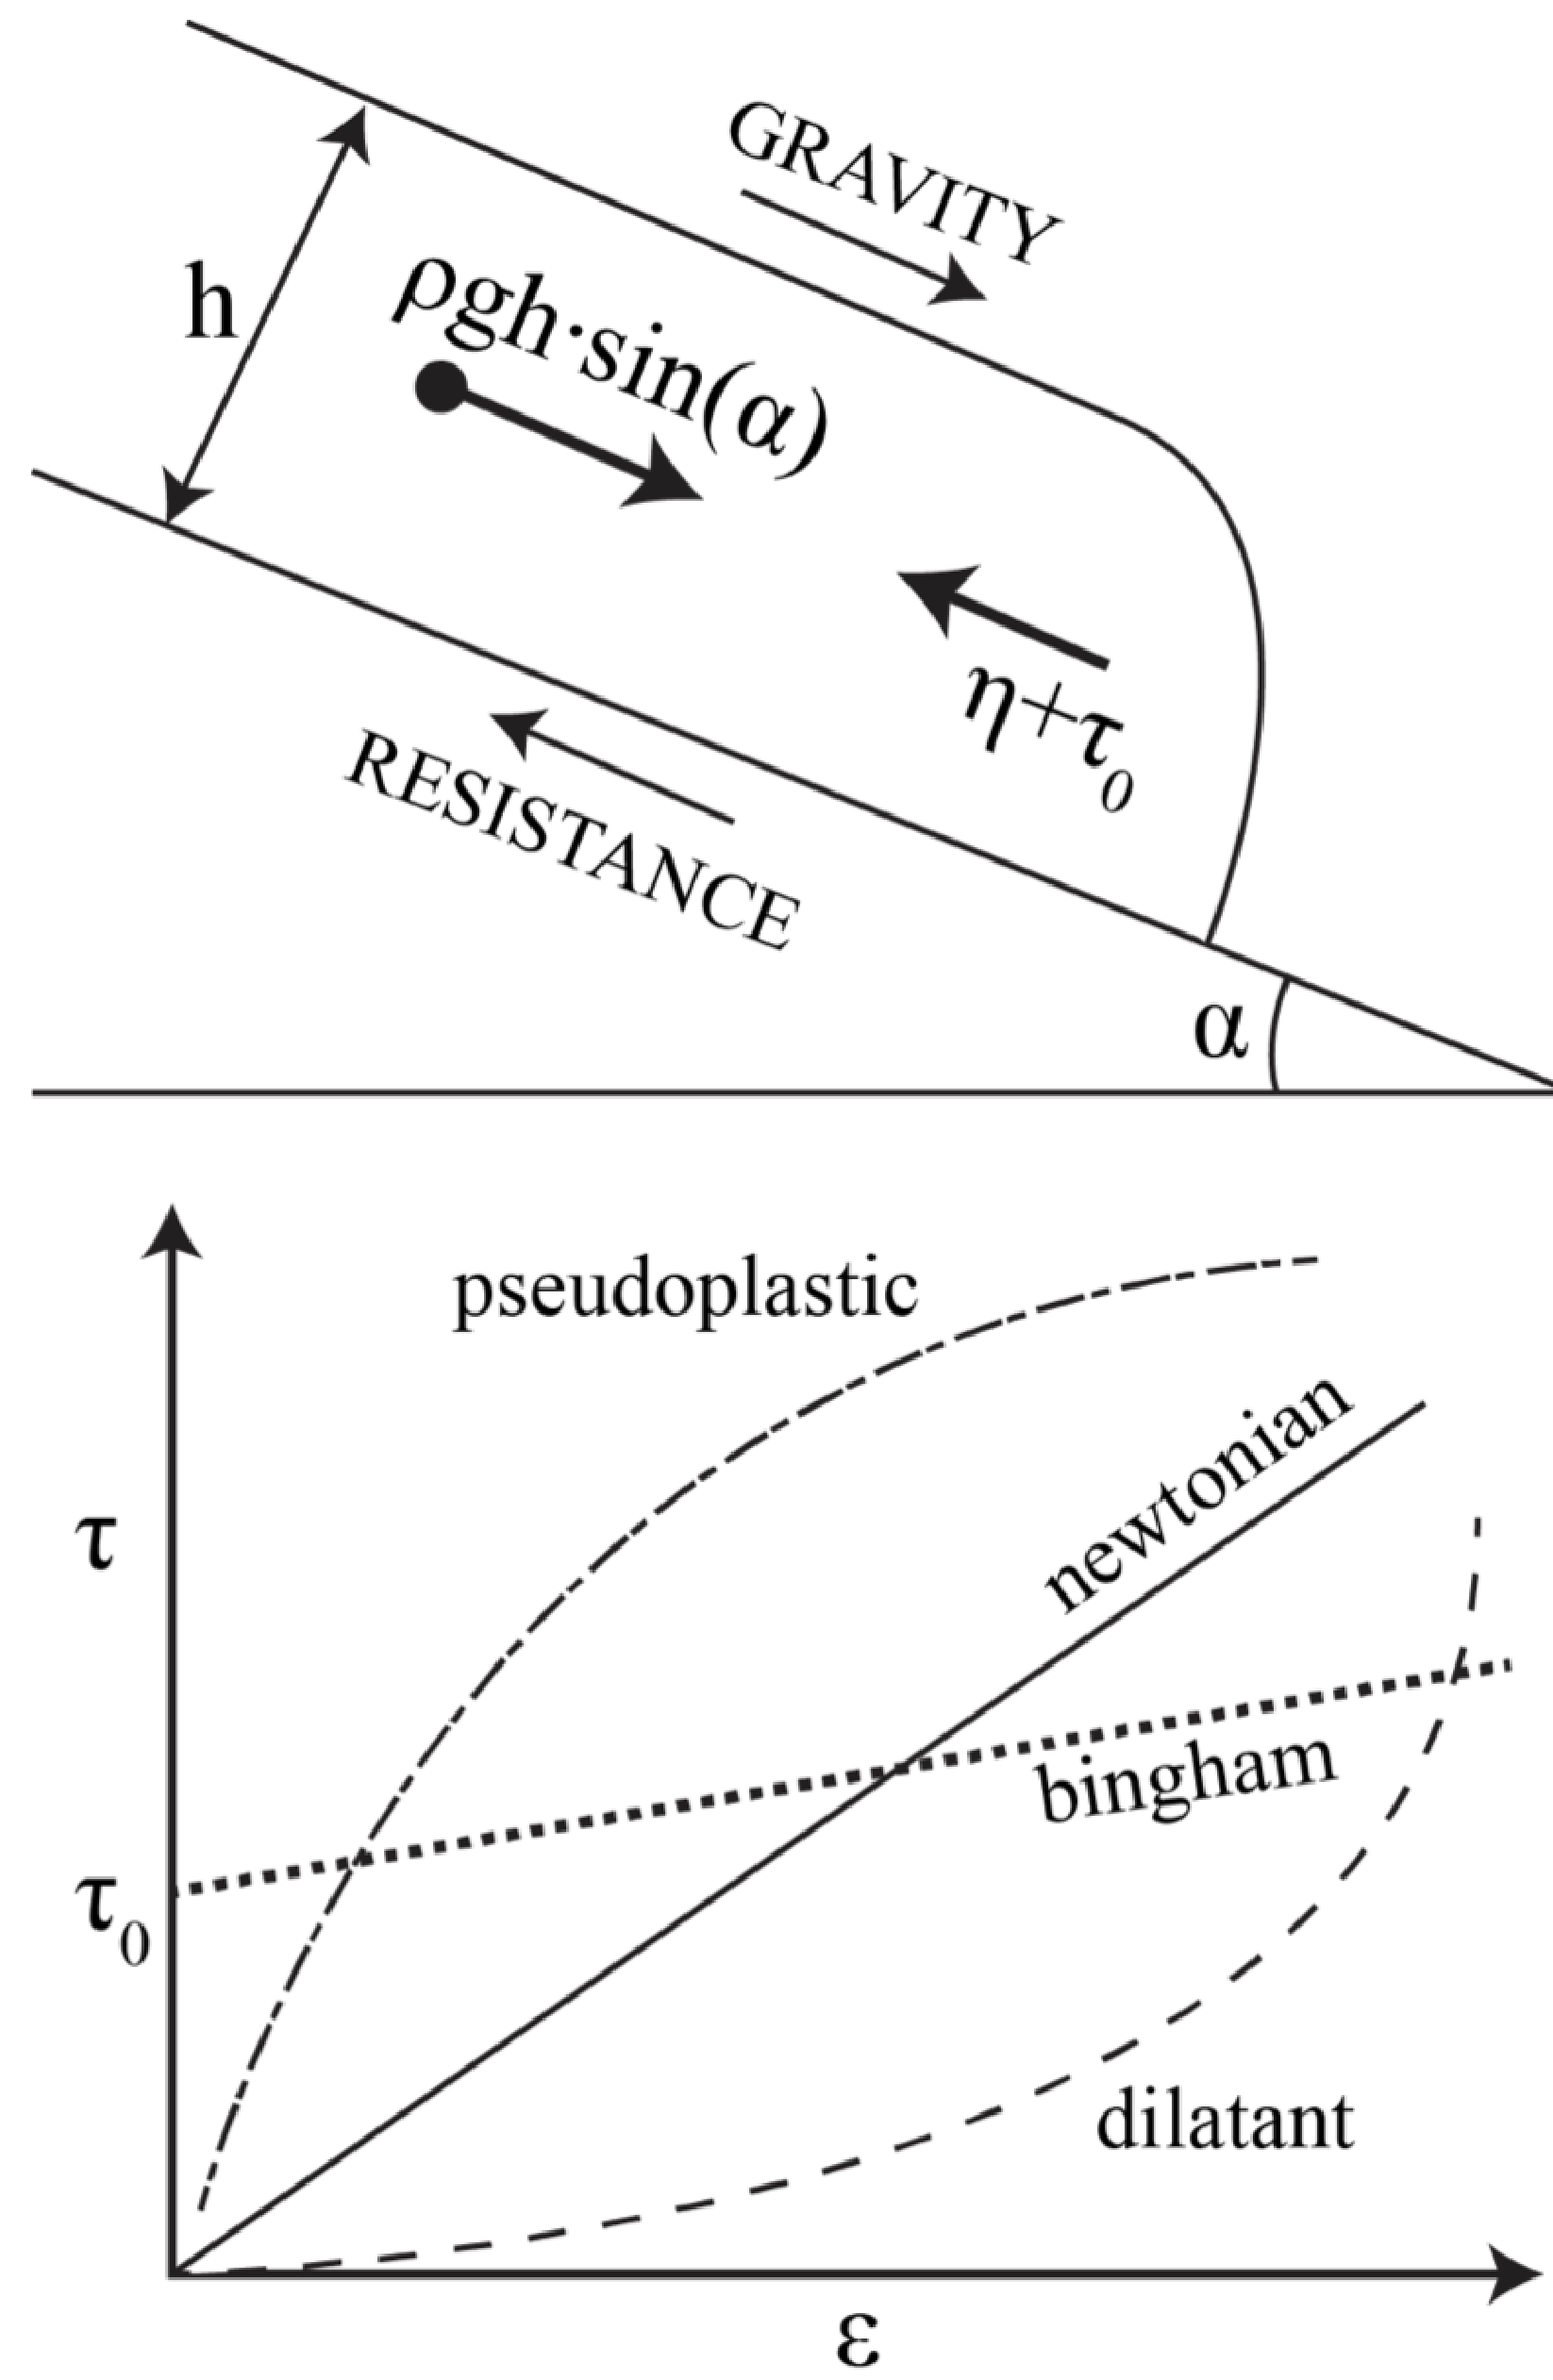
\includegraphics[width=1\textwidth]{img/rheology.png}
%       \end{column}
%     \end{columns}

    
% \end{frame}

% \begin{frame}{Flow types}

%     \begin{columns}[T]
%       \begin{column}{0.65\textwidth}	

%         \only<1-2>{
%           \textbf{Newtonian fluids}\\ \vspace*{.5em}
          
%           \begin{itemize}
%             \item Newtonian fluids start to flow/deform when an \alert{infinitesimally low shear stress is applied}
%             \item The relationship between the applied force ($\rightarrow$shear stress) and rate of deformation ($\rightarrow$strain rate) is \alert{linear}
%           \end{itemize}
          
%         }

%         \only<2>{
%           \textbf{Non-newtonian fluid}\\ \vspace*{.5em}
          
%           A fluid is non-newtonian when one of these conditions is met:
%           \begin{itemize}
%             \item The relationship between shear stress and strain rate is \alert{non-linear}
%             \item A \alert{yield strength must be exceeded} before flowing occurs, after which the shear stress/strain rate relationship can be linear or not
%           \end{itemize}
          
%         }

%         \only<3-4>{
%           \textbf{Non-newtonian fluid}\\ \vspace*{.5em}
          
%           Amongst non-newtonian fluids, fluids with variable shear stress/strain rate include:
%           \begin{itemize}
%             \item \textbf{Dilatant fluids}: apparent viscosity increases with increasing shear rate $\rightarrow$ \alert{shear thickening fluids}
%             % Cornstarch
%             \item \textbf{Pseudoplastic fluids}: apparent viscosity decreases with increasing shear rate $\rightarrow$ \alert{shear thinning fluids}
%             % Quicksand, ketchup
%           \end{itemize}
%         } 
%         \only<4>{
%           \vspace*{2em}
%           \textbf{Bingham fluids} are a special type of non-newtonian fluids characterized by a \alert{yield strength} and a \alert{linear shear stress/strain rate relationship}
%         }
%         % \only<5>{
          
%         %   \textbf{Lava flows:} \vspace*{2em}
%         %   \begin{itemize}
%         %     \item Non-newtonian
%         %     \item Pseudoplastic
%         %     \item Yield strength
%         %   \end{itemize}
%         % }

%       \end{column}

%       \begin{column}{0.35\textwidth}	
%         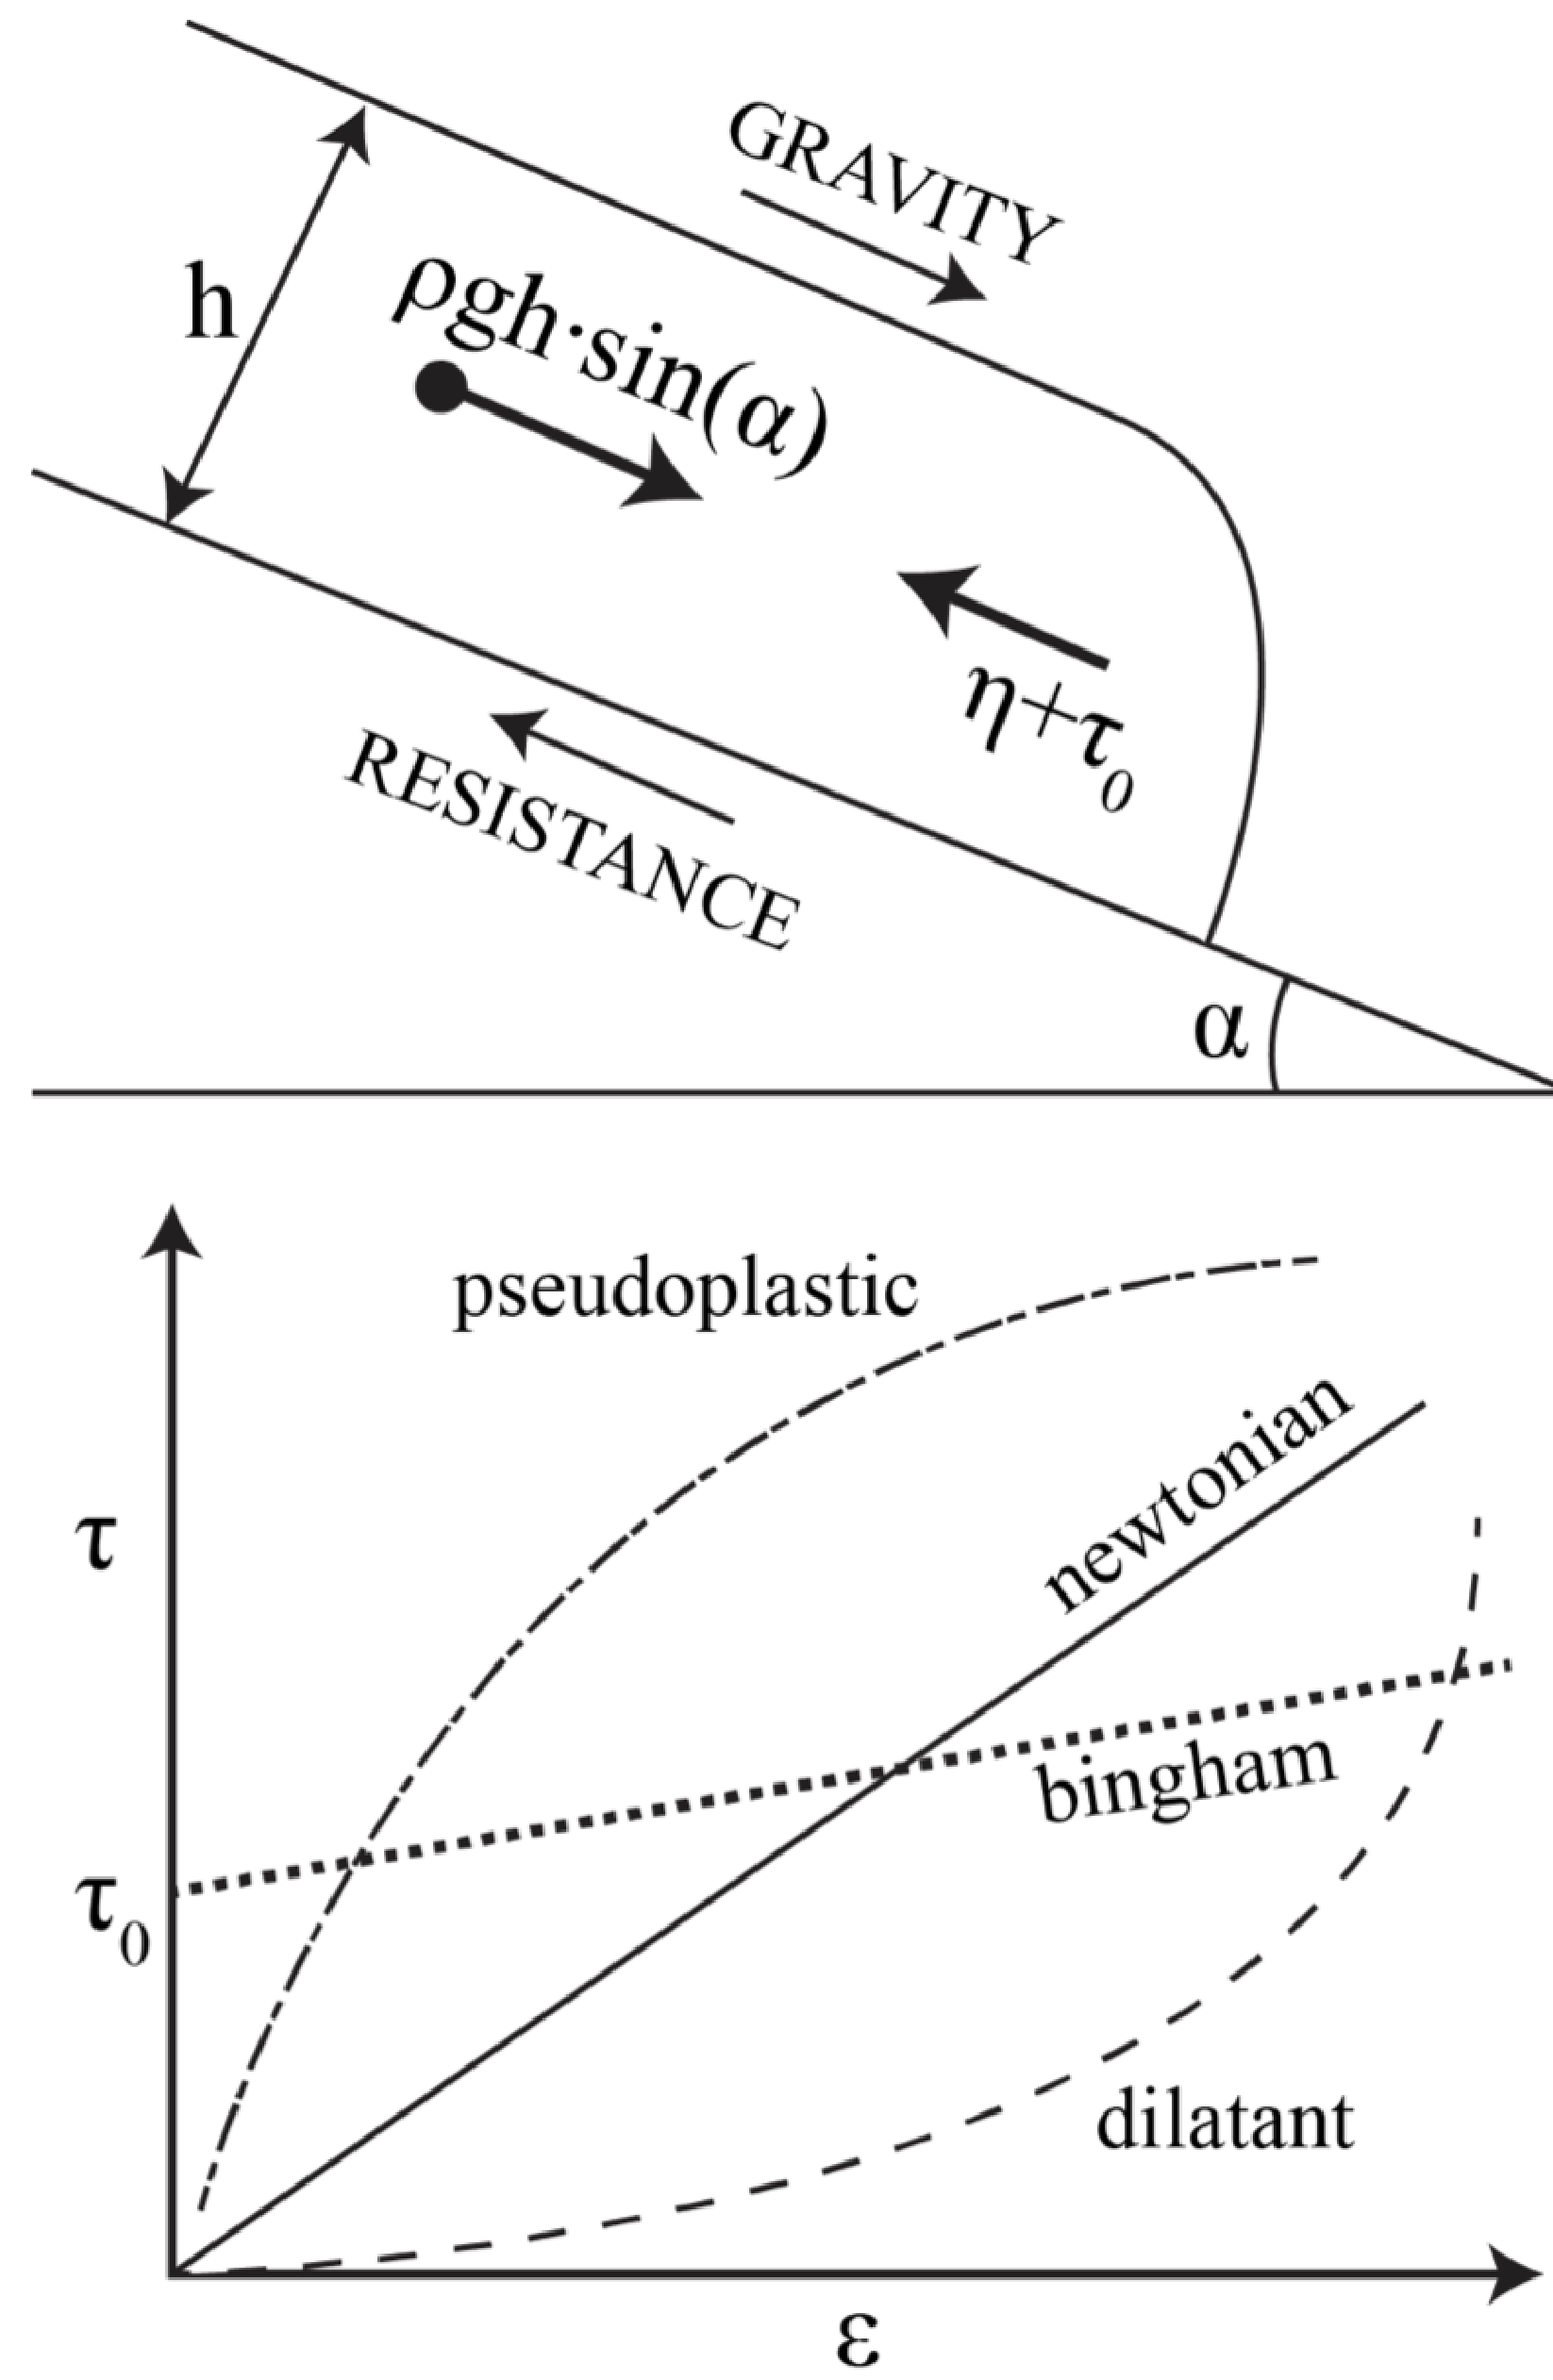
\includegraphics[width=1\textwidth]{img/rheology.png}
%       \end{column}
%     \end{columns}

    
% \end{frame}


% \begin{frame}[standout]
%   Experiment time!
% \end{frame}
 
% \begin{frame}[standout]
%   Movie time!
% \end{frame}

% \begin{frame}{Lava flow videos}
  
%   \textbf{Put these physical concepts in the perspective of actual lava flows!}\\
%   Look at these videos, and describe them in terms of:

%   \begin{itemize}
%     \item Flow \alert{shape}, \alert{geometry}, \alert{morphology}, \alert{texture}
%     \item \alert{Colour} (as an indicator to which physical parameter)
%     \item \alert{Velocity} and flow rate
%     \item \alert{Driving} and \alert{resisting} forces
%   \end{itemize} 
  
%   \vspace*{2em}
%   \textbf{What type of fluid are \alert{lava flows}?}
% \end{frame}


% \begin{frame}[standout]
%   \alert{Conclusion:} It is slightly more complicated...
% \end{frame}


% \begin{frame}{Case study: the 2016 61G flow}
  
%   \only<1>{ 
%     \begin{columns}[T]
%       \begin{column}{0.5\textwidth}	
%         \centering \includegraphics[width=1\textwidth]{../docs/img/61g/HI.png}
%       \end{column}

%       \begin{column}{0.5\textwidth}	
%         \centering 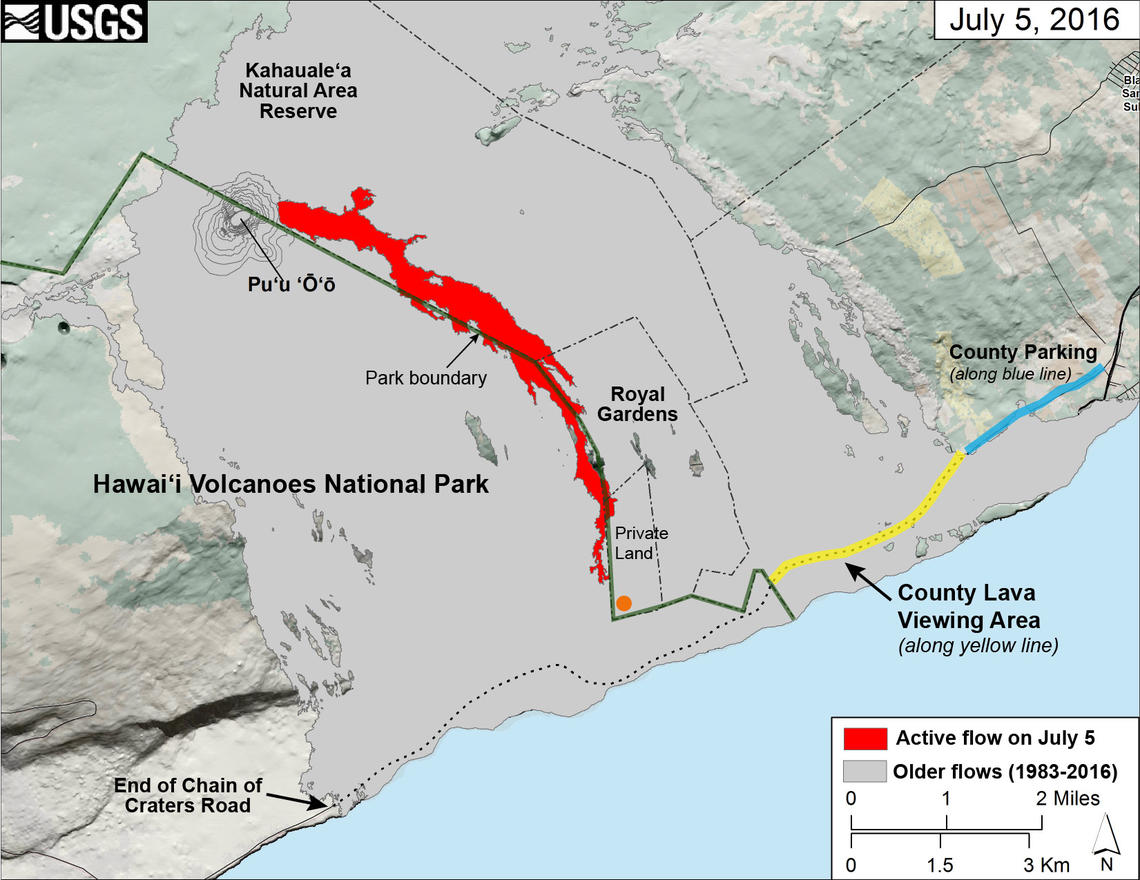
\includegraphics[width=1\textwidth]{../docs/img/61g/61g.jpg}
%       \end{column}
%     \end{columns}
%   }
%   \only<2>{
%     \centering Pahoehoe toes $\rightarrow$ \alert{Thermal insulation} $\rightarrow$ Lava tube
%     \begin{columns}[T]
%       \begin{column}{0.5\textwidth}	
%         \centering 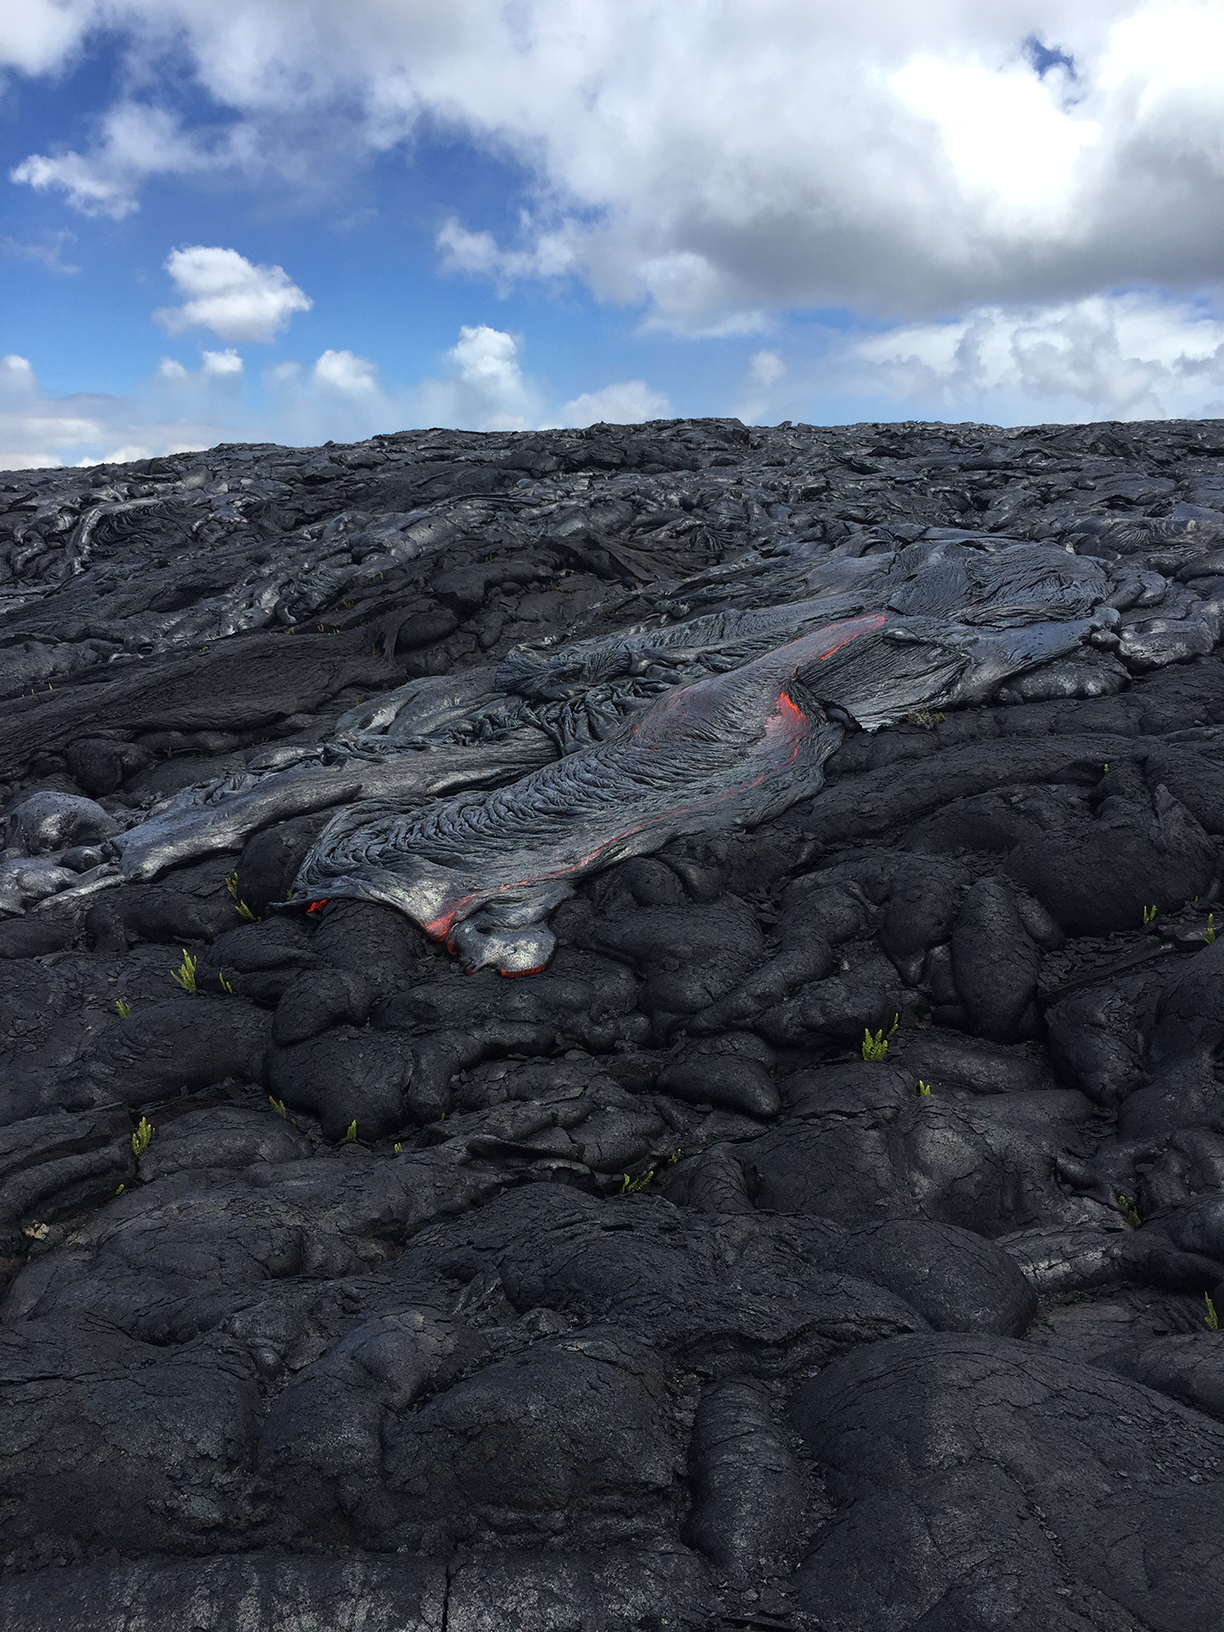
\includegraphics[width=.8\textwidth]{../docs/img/61g/toes.png}
%       \end{column}

%       \begin{column}{0.5\textwidth}	
%         \centering 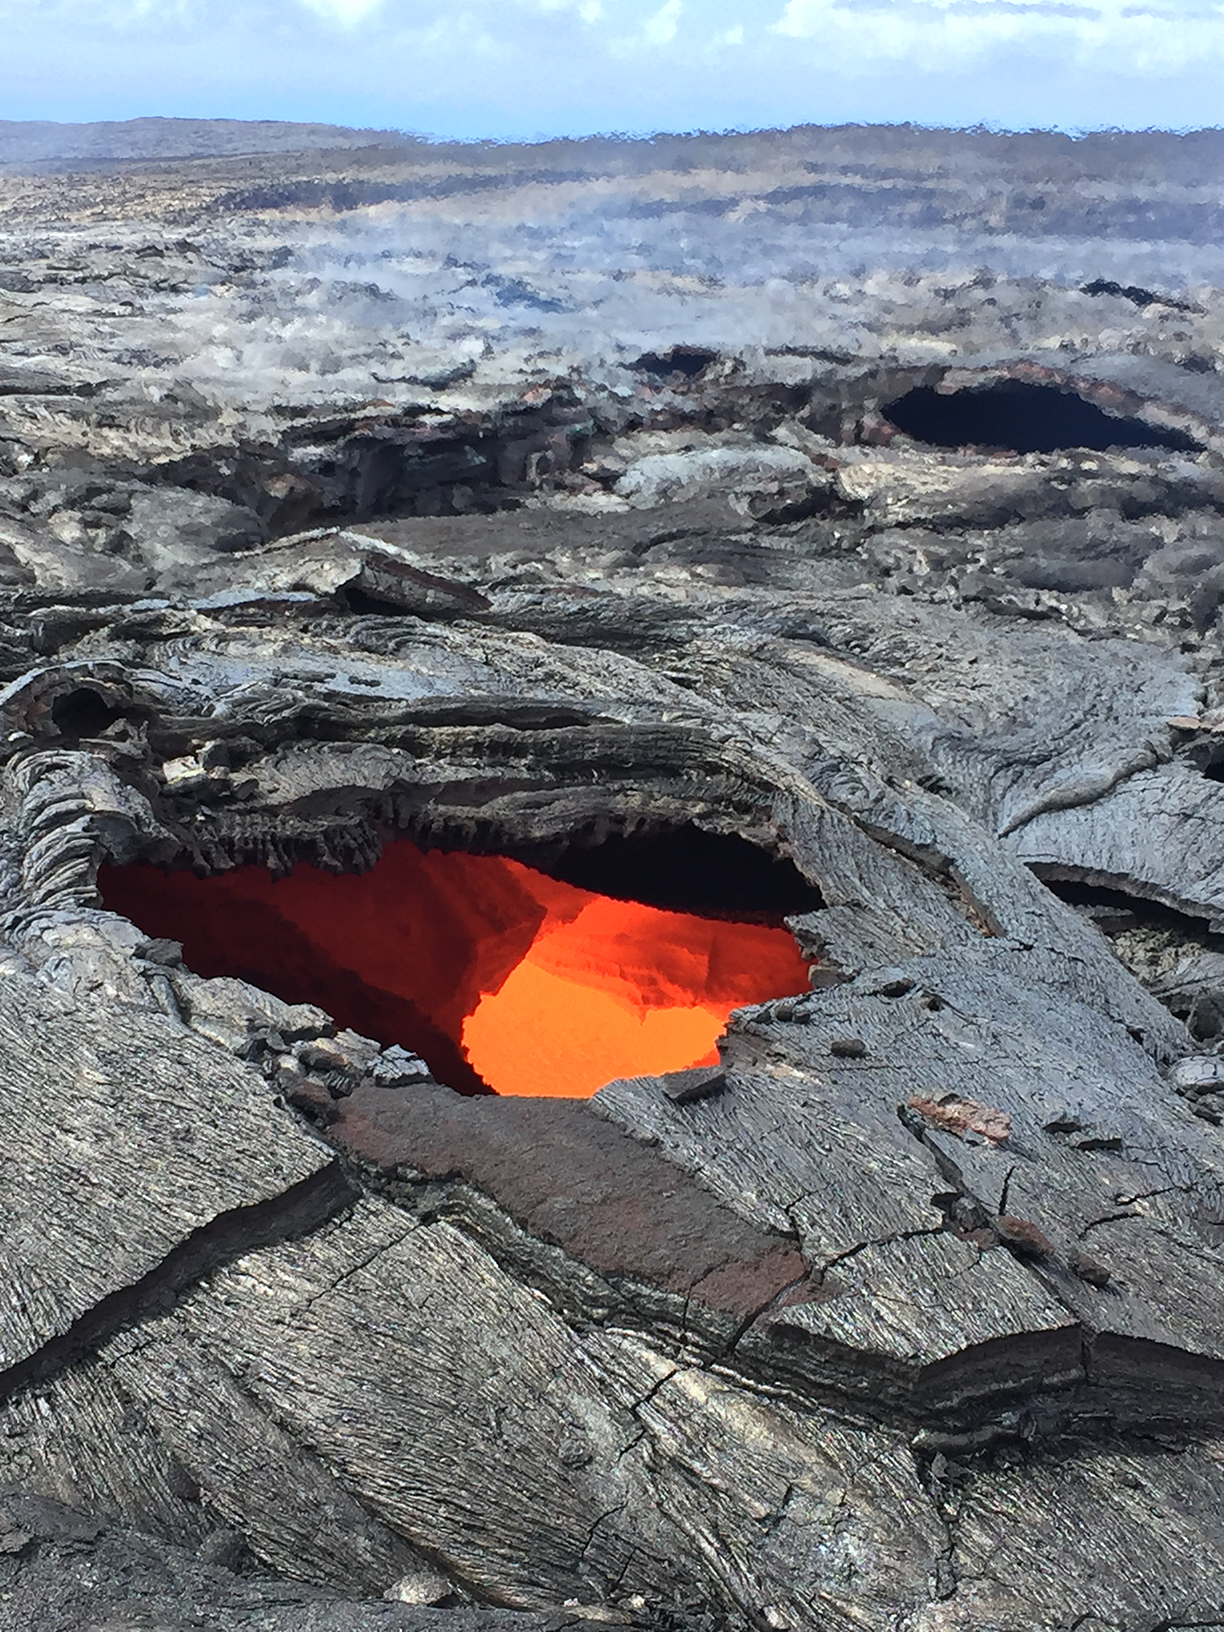
\includegraphics[width=.8\textwidth]{../docs/img/61g/tube.png}
%       \end{column}
%     \end{columns}
%   }
%   \only<3>{
%     \centering Morphology transition $\rightarrow$ \alert{Topography}
%     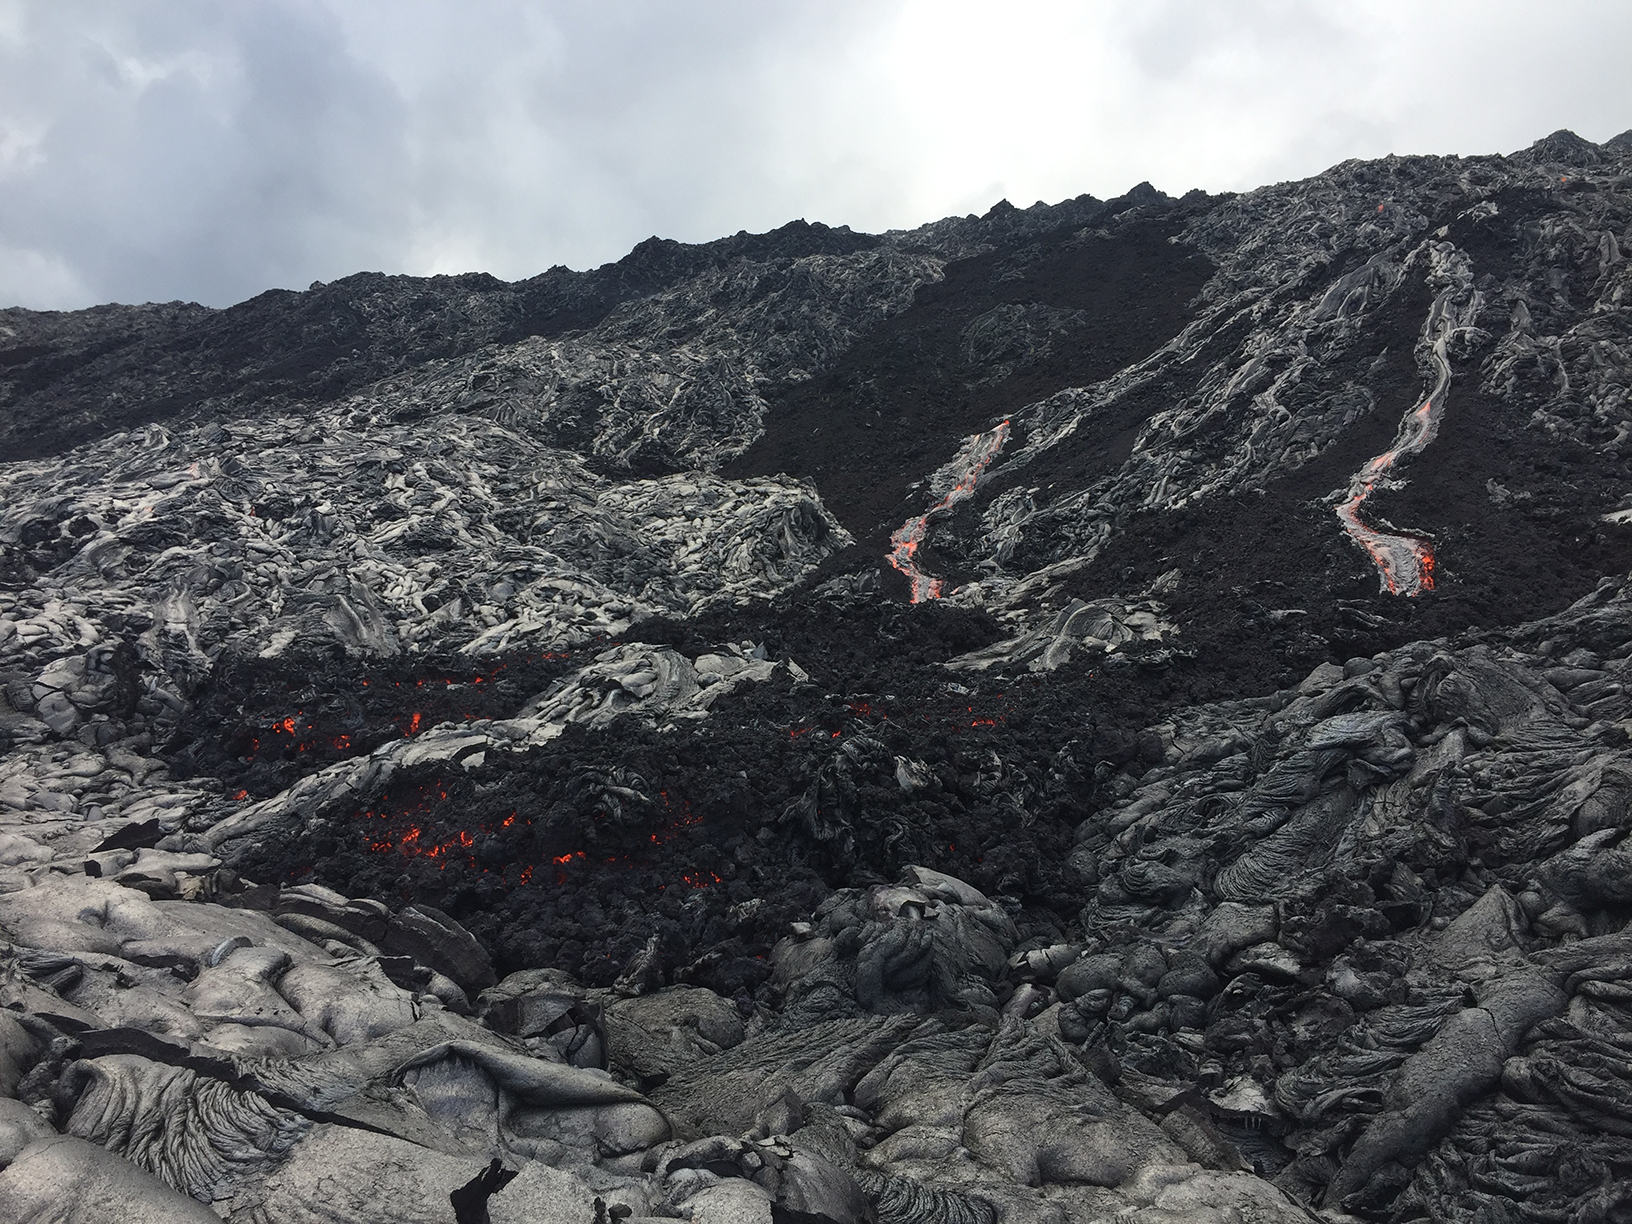
\includegraphics[width=.8\textwidth]{../docs/img/61g/pali.png}
%   }
%   \only<4>{
%     \centering Structure-from-motion $\rightarrow$ \alert{DEM evolution}\vspace*{.8em}
%     \includegraphics[width=.8\textwidth]{../docs/img/61g/DEM.png}
%     }
%   \only<5>{
%     \centering DEM evolution $\rightarrow$ \alert{Validation of steepest descent}\vspace*{.8em}
%     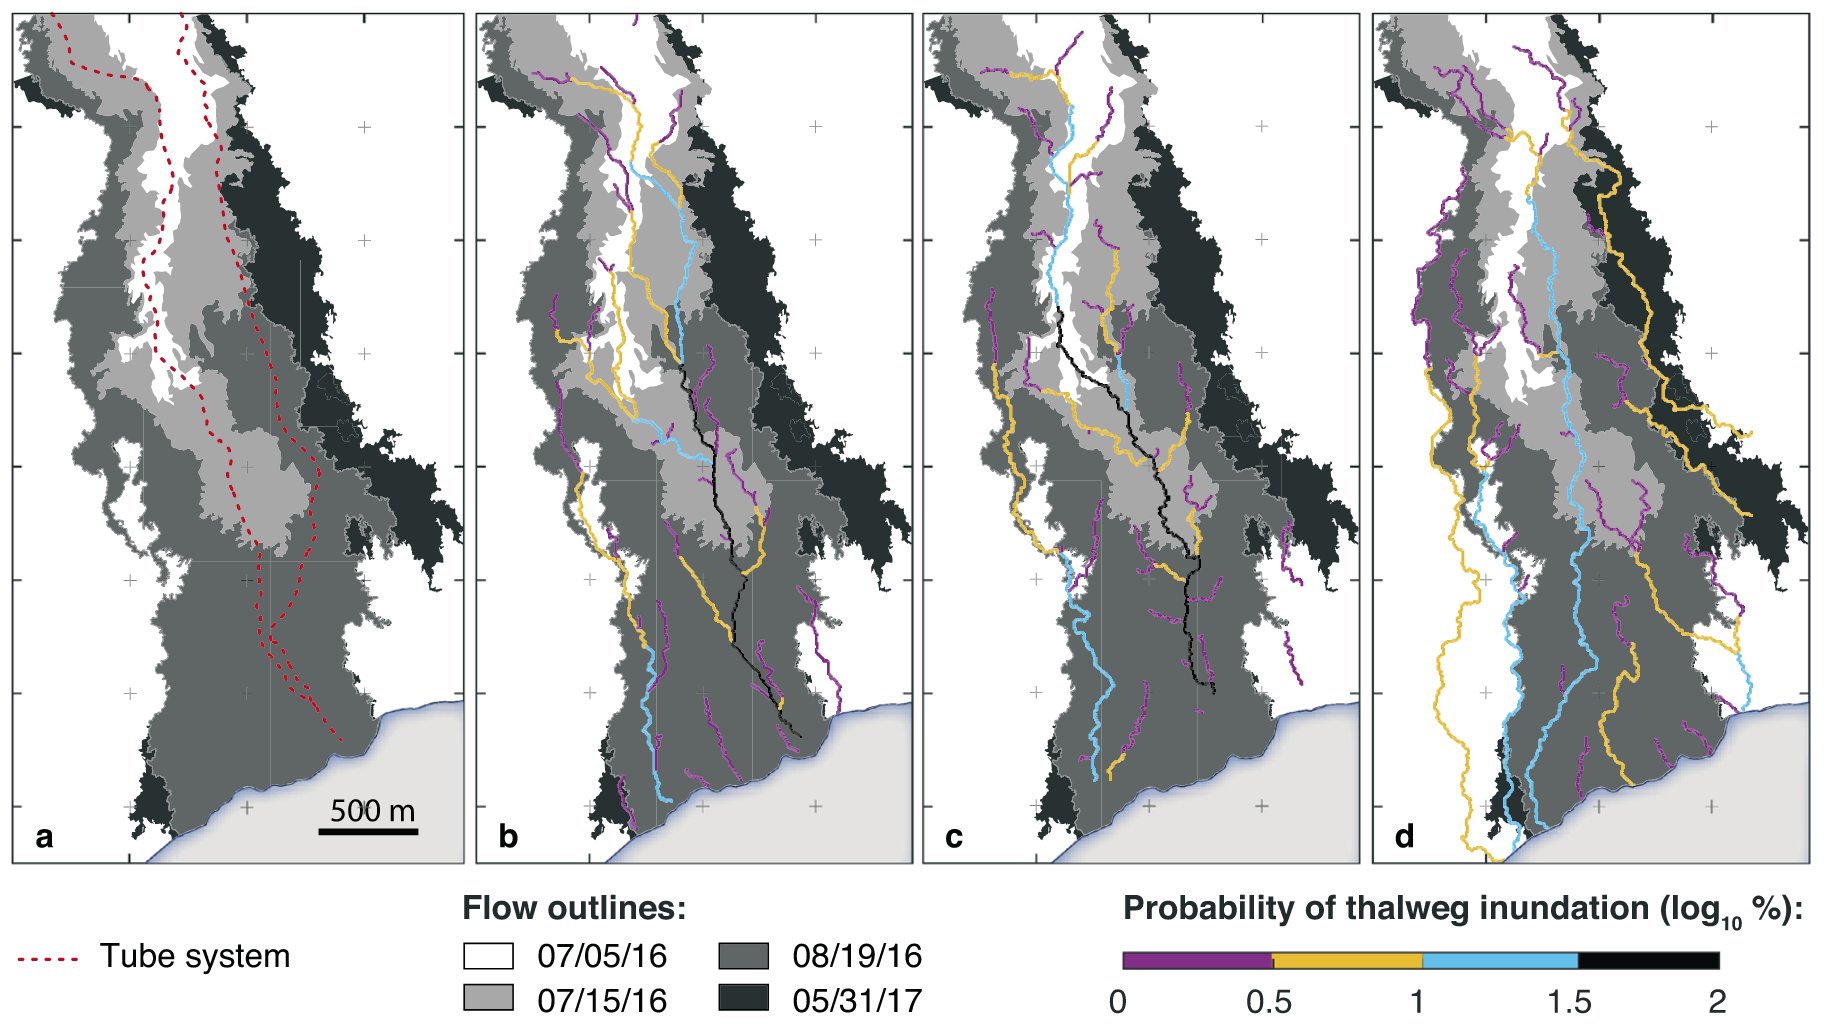
\includegraphics[width=.9\textwidth]{../docs/img/61g/steepest.png}
%   }
%   \only<6>{
%     \centering Thermal imagery $\rightarrow$ \alert{Heat budget}\vspace*{.8em}
%     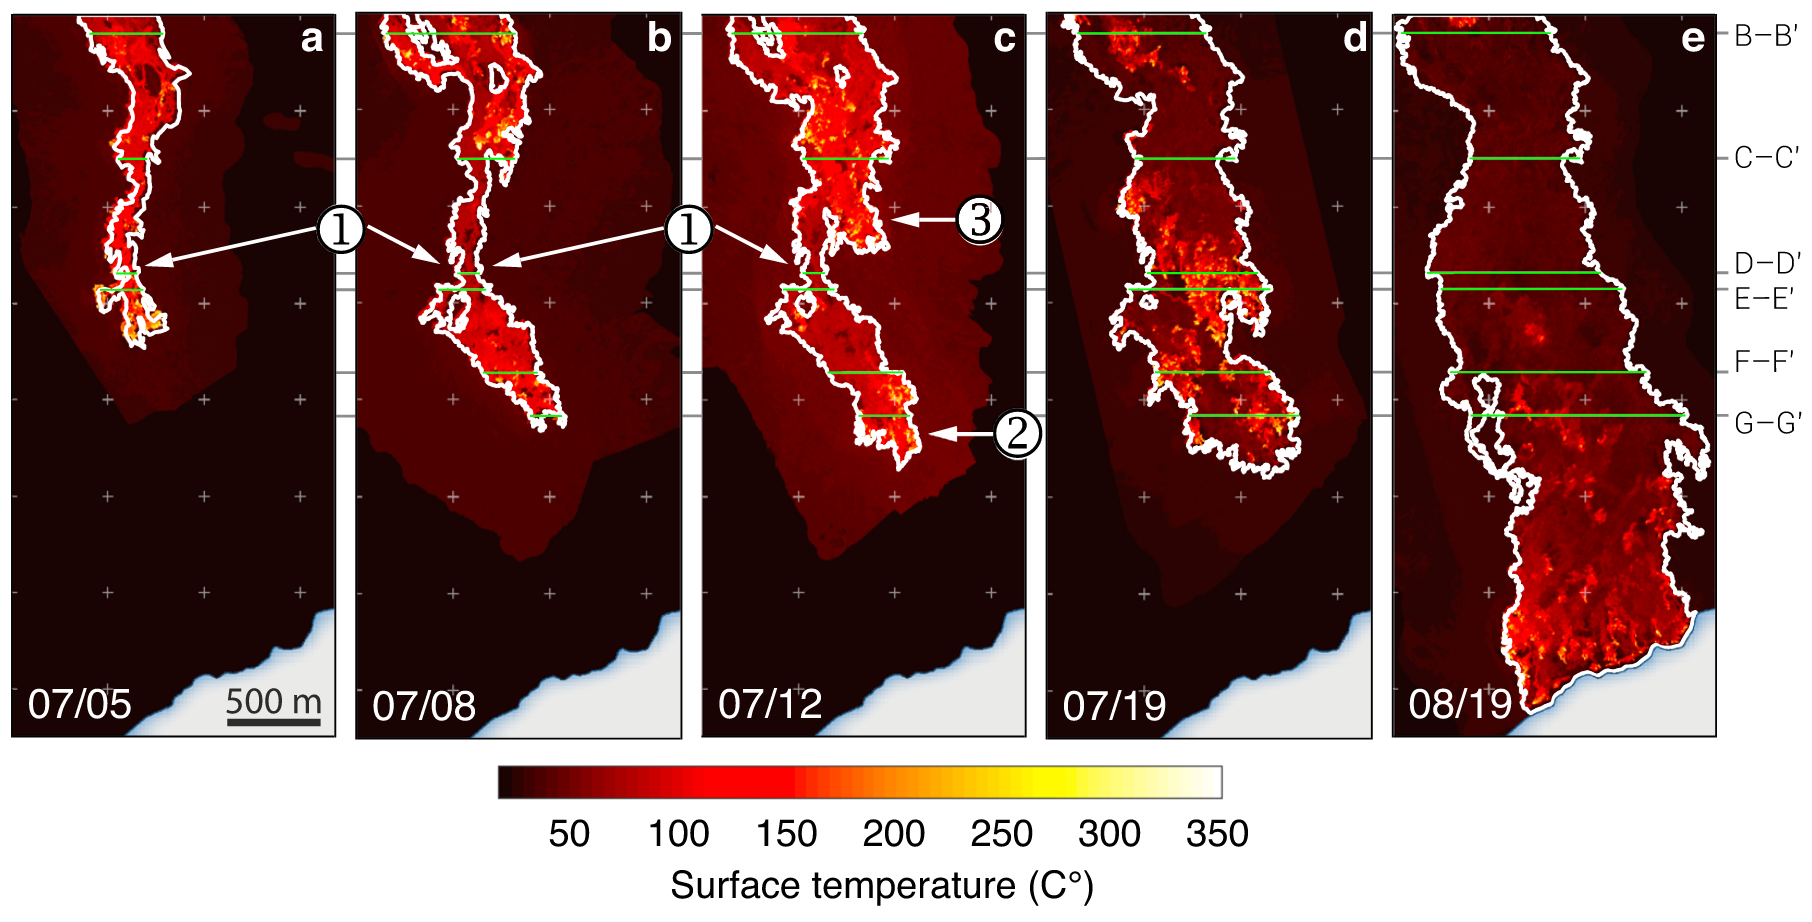
\includegraphics[width=1\textwidth]{../docs/img/61g/thermal.png}
%   }
% \end{frame}


% \begin{frame}{Perspective}
%   \only<1>{
%     Lava flows often result in \alert{long--lasting crises} characterised by \alert{large uncertainties}. This is partly the case because:
%     \begin{itemize}
%       \item Lava flows are \alert{too complex} to (currently) be fully described by physical models 
%       \begin{itemize}
%         \item[$\rightarrow$] Spatio-temporal evolution of parameters affecting rheology,
%         \item[$\rightarrow$] Interaction with environment, stochastic processes
%       \end{itemize}
%       \item Need a framework to \alert{account for}, \alert{quantify} and \alert{communicate} \textbf{uncertainties}
%       \begin{itemize}
%         \item[$\rightarrow$] \alert{Epistemic} vs \alert{aleatory}
%       \end{itemize}
%     \end{itemize}
%     }
%   \only<2>{
%     \centering \alert{\textit{"A simple, imperfect model is better than no model"}}\\ \vspace*{1em}
%     \centering \alert{\textit{"All models are wrong, but some are useful"}}\\ \vspace*{1em}

%     \centering \begin{itemize}
%       \item[$\rightarrow$] A lot of models are available (see \alert{Resources} page) \textbf{but}
%       \item[$\rightarrow$] They require understanding \alert{limitations} and \alert{sources of uncertainties}
%     \end{itemize}
%   }

% \end{frame}

% \section{\alert{Lava flow part III} \\ Probabilistic modeling}

% \begin{frame}{Vent location}
%     \begin{columns}[T]
%       \begin{column}{0.5\textwidth}	
%         \centering \textbf{Monogenetic vents}\\ \vspace*{1em}
%         \centering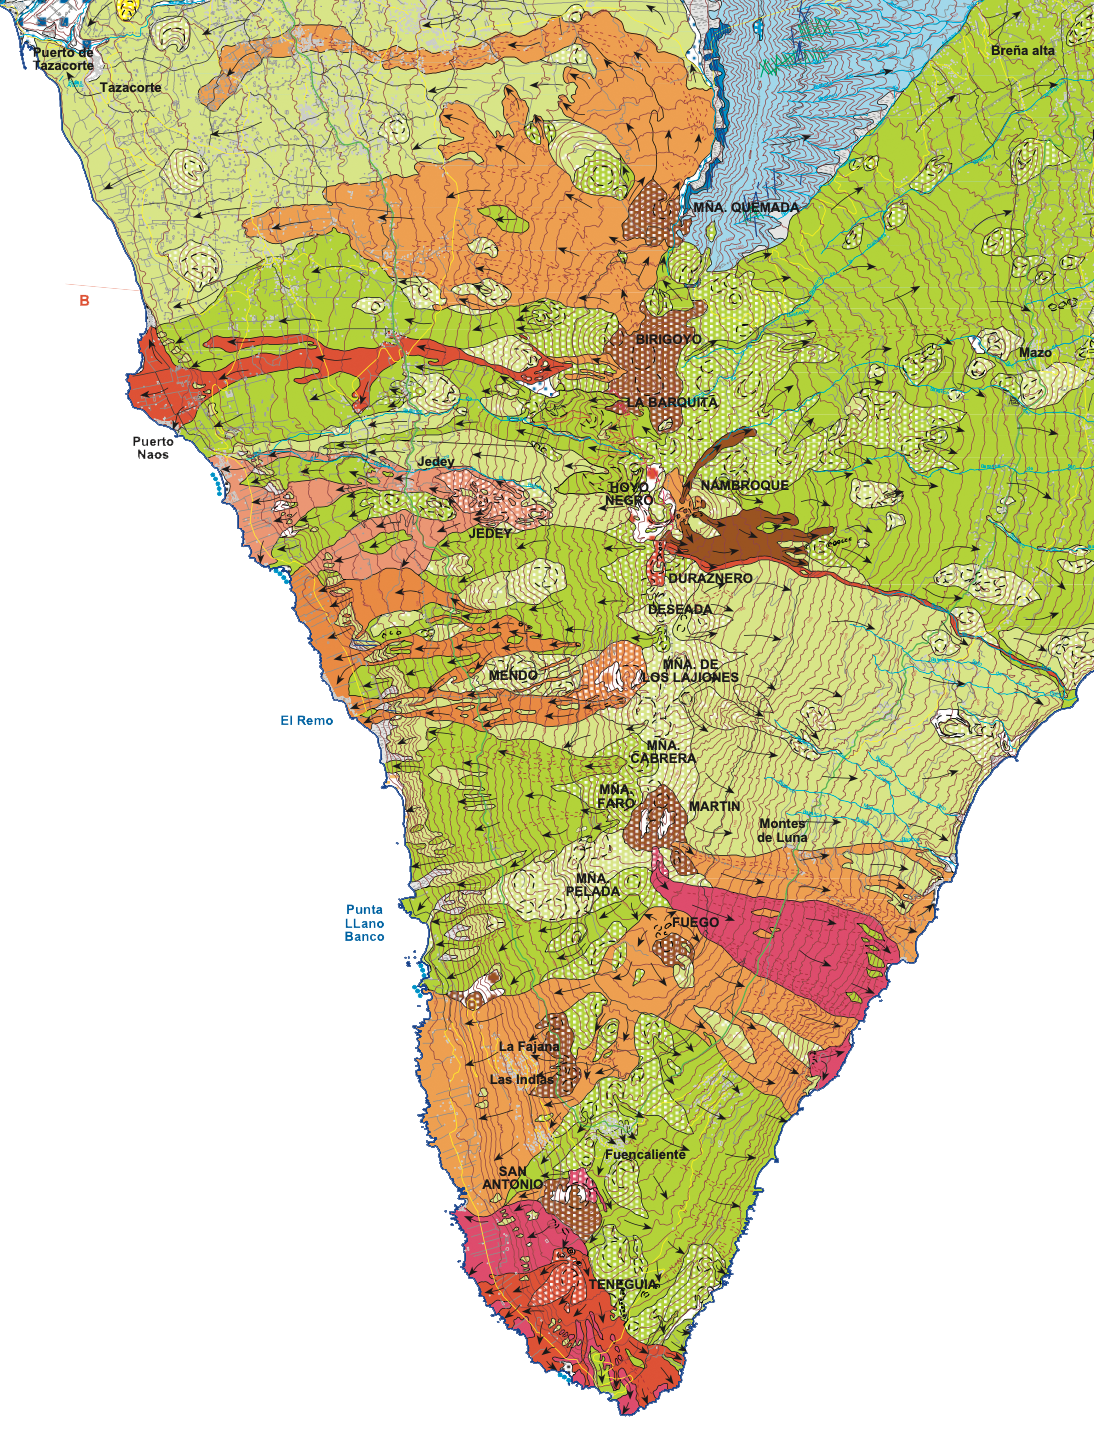
\includegraphics[width=.85\textwidth]{img/lapalma.png}
%       \end{column}

%       \only<1>{
%       \begin{column}{0.5\textwidth}	
%         \centering \textbf{Future eruptions}\\ \vspace*{1em}
%         \centering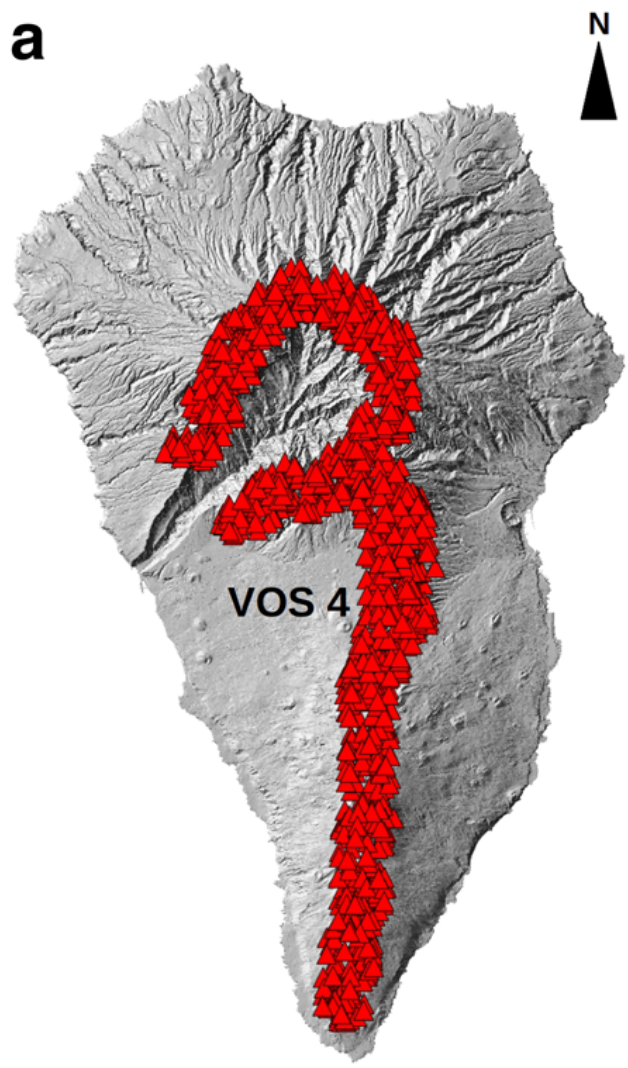
\includegraphics[width=.55\textwidth]{../docs/img/hydro/Marrero_vents.png}
%       \end{column}
%       }
%       \only<2>{
%       \begin{column}{0.5\textwidth}	
%         \centering \textbf{Multiple vents for one eruptions}\\ \vspace*{1em}
%         \centering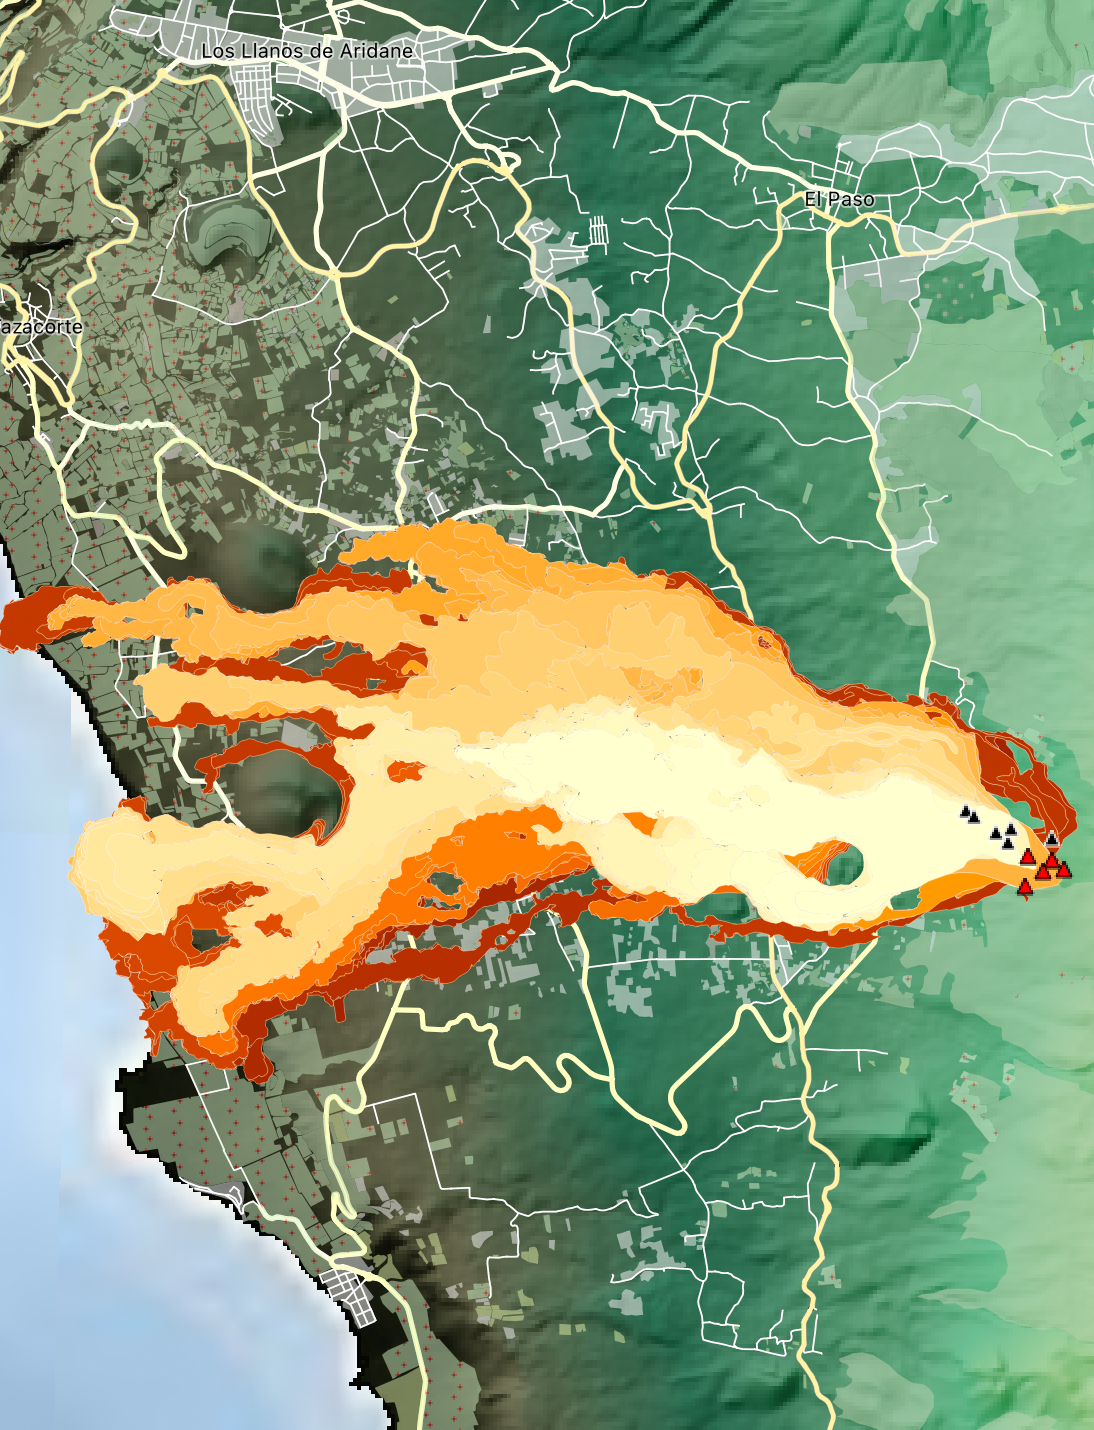
\includegraphics[width=.85\textwidth]{img/lapalma_2.png}
%       \end{column}
%       }
%     \end{columns}
%  \end{frame}

% \begin{frame}[standout]
%   How do we account for the \alert{uncertainty on vent location} in our hazard assessment for lava flow inundation?
% \end{frame}

% \begin{frame}[t]{Exploring vent location...}
%   ...using a frequentist approach:
%   \begin{columns}[T]
%     \begin{column}{0.5\textwidth}
      
%       \begin{enumerate}
%         \item<1- | alert@1> Assumption that a new vent can open from all these vents
%         \begin{itemize}
%           \item[$\rightarrow$]<1-> For now, assume \textit{equal probability}
%         \end{itemize}
%         \item<2- | alert@2> Run \textit{path of steepest descent} from all vents
%         \begin{itemize}
%           \item[$\rightarrow$]<2-> Some pixels are \textit{more likely} to be inundated
%         \end{itemize}
%         \item<3- | alert@3> Count the \textbf{number of times} a given pixel is inundated and \textbf{normalise} by the number of vents
%       \end{enumerate}

%     \end{column}

%     \begin{column}{0.5\textwidth}	
%       \only<1>{
%         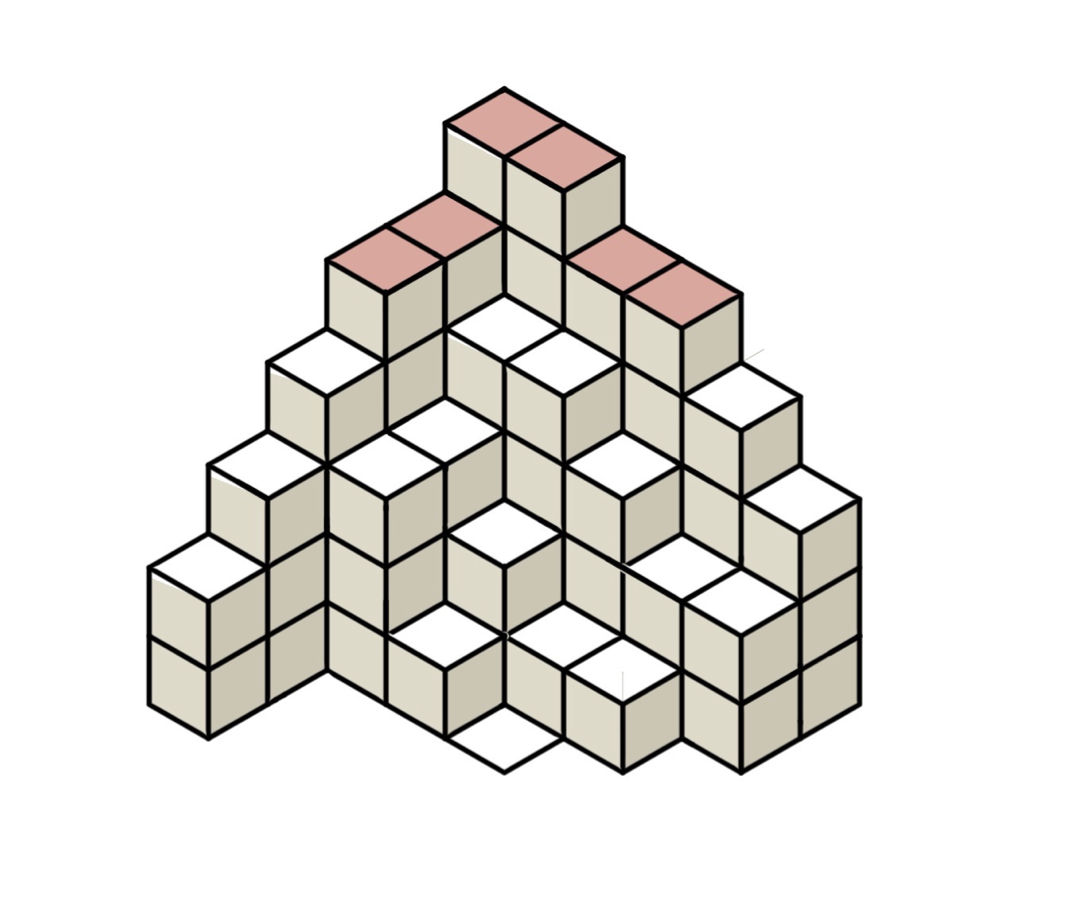
\includegraphics[width=1\textwidth]{../docs/img/hydro/prob1.png}
%       }
%       \only<2>{
%         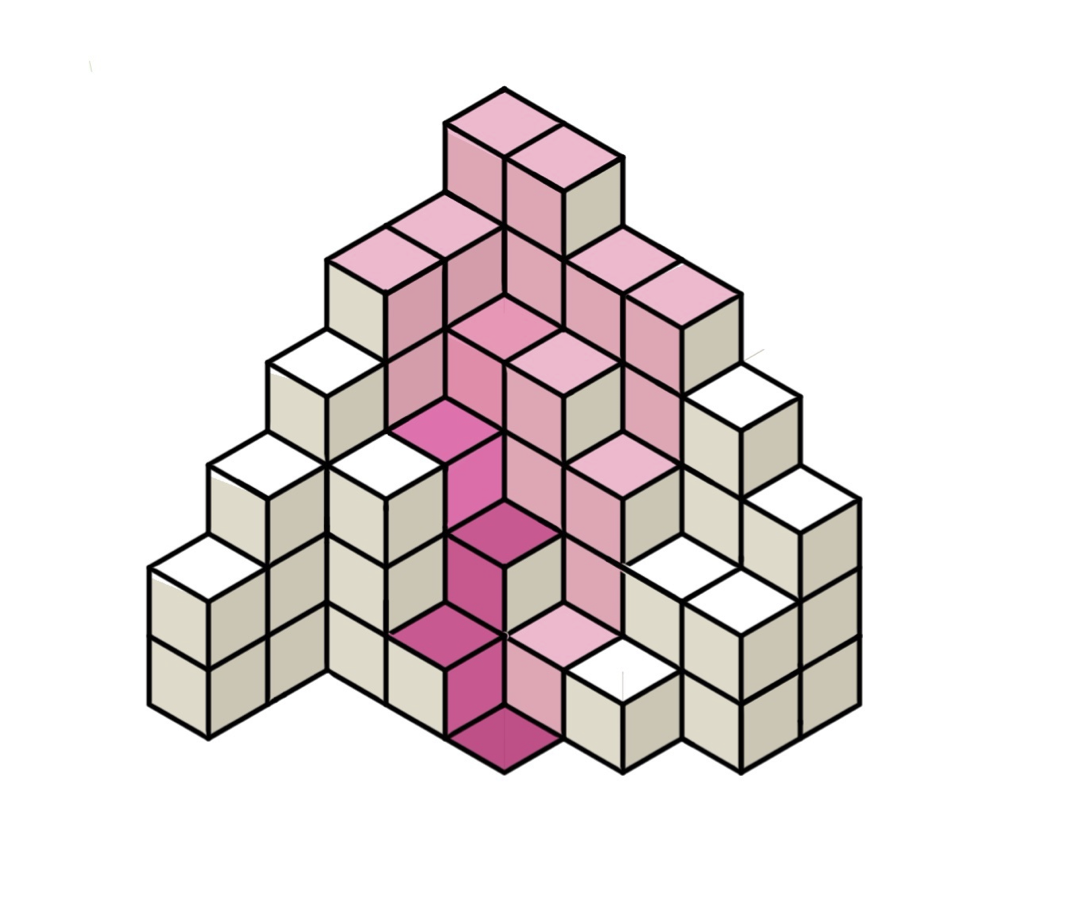
\includegraphics[width=1\textwidth]{../docs/img/hydro/prob2.png}
%       }
%       \only<3>{
%         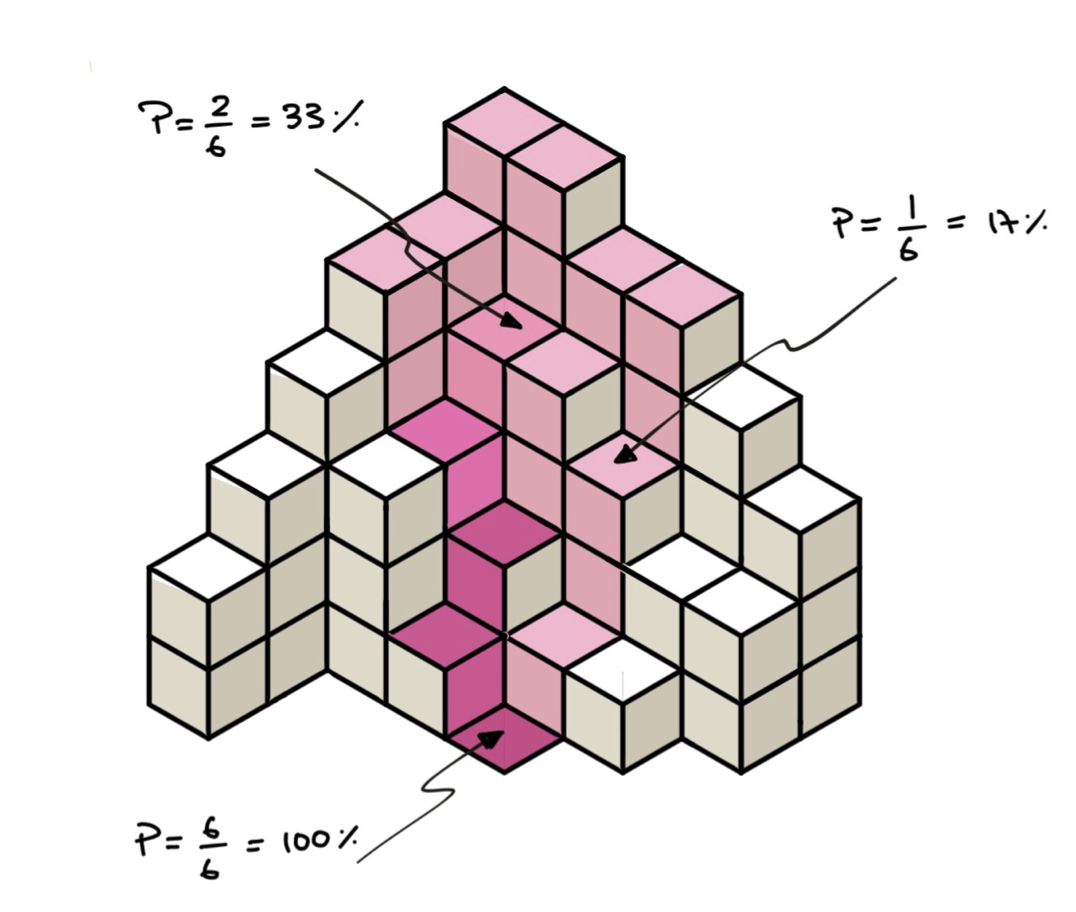
\includegraphics[width=1\textwidth]{../docs/img/hydro/prob3.png}
%       }
%     \end{column}
%   \end{columns}
% \end{frame}

% \begin{frame}[t]{Deterministic vs probabilistic modeling}
%   \only<1-2>{
%   \begin{columns}[T]
%     \begin{column}{0.5\textwidth}
      
%       \only<1>{
%         \centering \textbf{Deterministic scenario}\\ \vspace*{1.2em}

%         \centering 
%         \alert{One} user-defined value for each model input \\
%         $\downarrow$\\
%         \alert{One} model run\\
%         $\downarrow$\\
%         \alert{One} possible outcome
%       }

%       \only<2>{
%         \centering \textbf{Probabilistic scenario}\\ \vspace*{1.2em}

%         \centering 
%         \alert{Range} of values as model inputs \\
%         $\downarrow$\\
%         \alert{Many model runs} with input conditions \alert{sampled} in input ranges\\
%         $\downarrow$\\
%         Aggregation of \alert{all possible outcomes} into \alert{probabilities}\\ \vspace*{.8em}
%         $\downarrow$\\ \vspace*{.8em}
%         \textbf{Allows exploring:}\\
%         $\rightarrow$ \alert{Uncertainties} on input parameters\\
%         $\rightarrow$ What \alert{could} happen in the future
%       }

%     \end{column}

%     \begin{column}{0.5\textwidth}	
%       \only<1>{
%        \centering 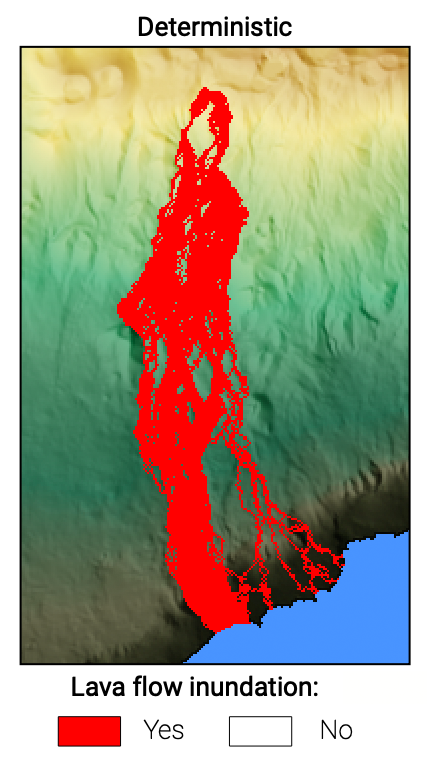
\includegraphics[width=.575\textwidth]{img/lava_dt.png}
%       }
%       \only<2>{
%        \centering 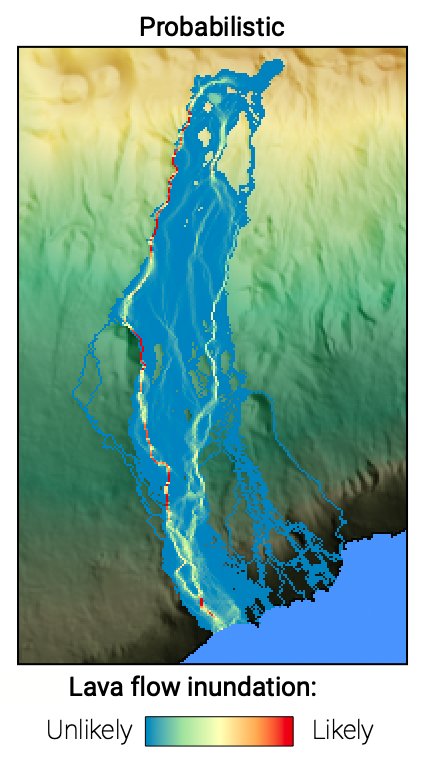
\includegraphics[width=.575\textwidth]{img/lava_prob.png}
%       }

%     \end{column}
%   \end{columns}
%   }
%   \only<3>{
%     \centering 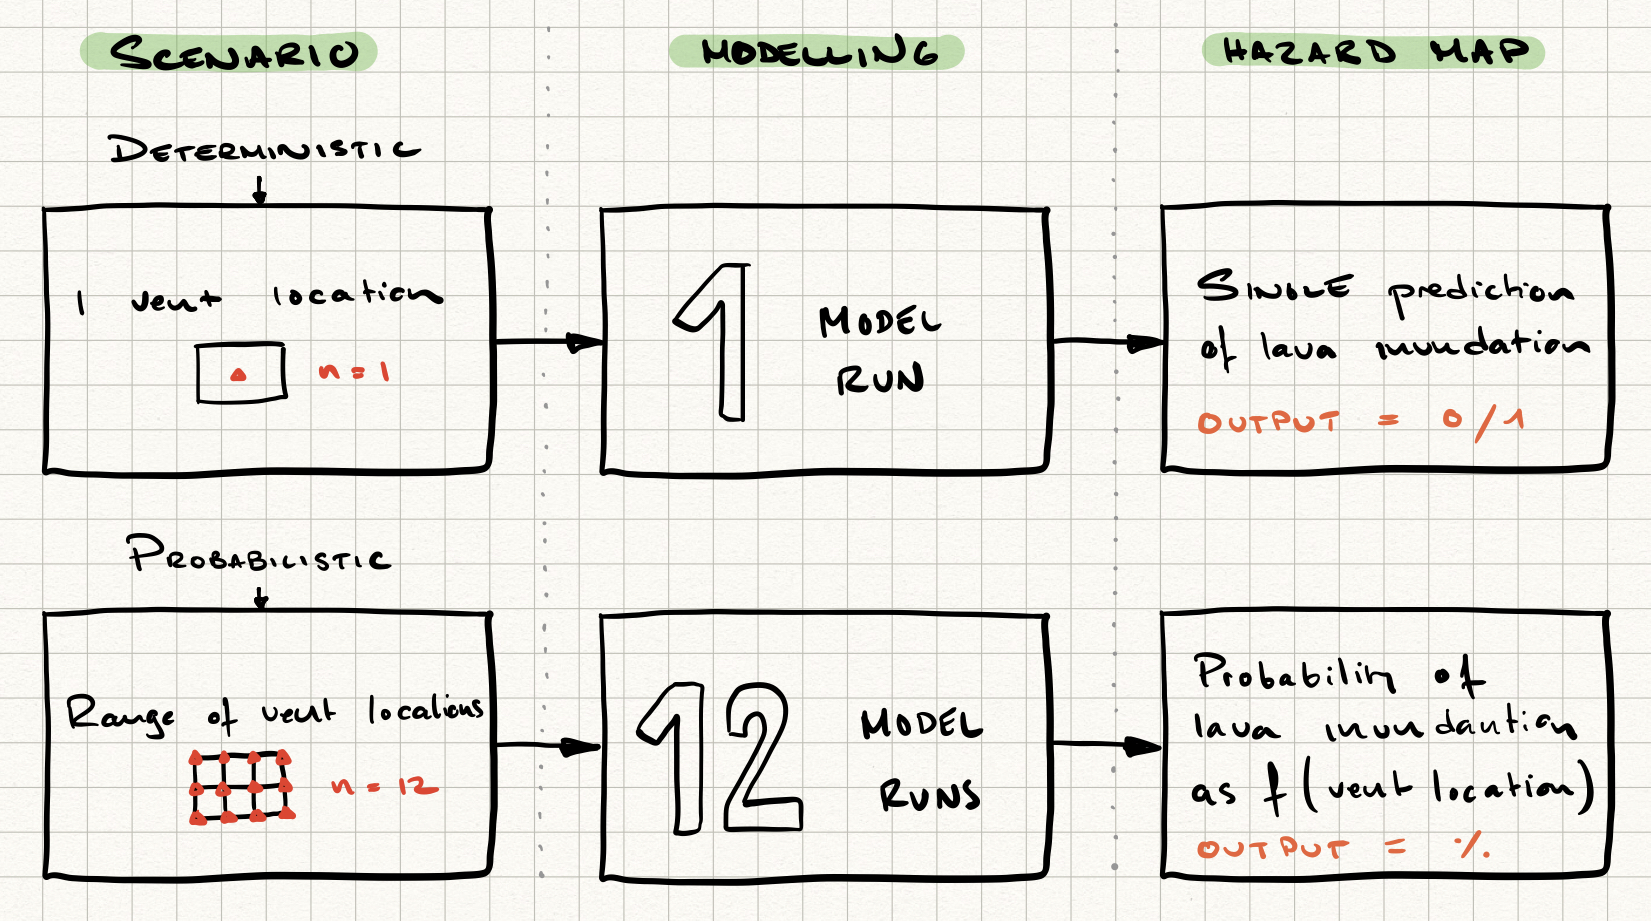
\includegraphics[width=.9\textwidth]{../docs/img/prob/prob1_wf.jpeg}
%   }


% \end{frame}


% \section{\alert{Lava flow part IV} \\ Q-LavHA}

% \begin{frame}{Q-LavHA}
%     \begin{columns}[T]
%       \begin{column}{0.5\textwidth}	
%         \begin{itemize}
%           \item<1- | alert@1> \textbf{Q-LavHA} $\rightarrow$ QGIS plugin
%           \item<1- | alert@1> Starting point $\rightarrow$ path of steepest descent
%           \item<2- | alert@2> Probabilistic approach to simulate:
%           \begin{itemize}
%             \item Flow \alert{inflation} $\rightarrow$ \alert{filling} depressions $\rightarrow$ lateral \alert{spreading}
%             \item Uncertainty on \alert{vent location}
%           \end{itemize}
%           \item<3- | alert@3> \alert{Thousands} of iteration of the path of steepest descent
%           \begin{itemize}
%             \item Next inundated pixel not only based on $\vert \Delta Z\vert $, but on a probability function based on $\vert \Delta Z\vert $ of all adjacent pixels
%           \end{itemize}
%           \item<4- | alert@4> \textbf{Output:} probability of flow inundation

%         \end{itemize}
%       \end{column}

%       \begin{column}{0.5\textwidth}	
%         \centering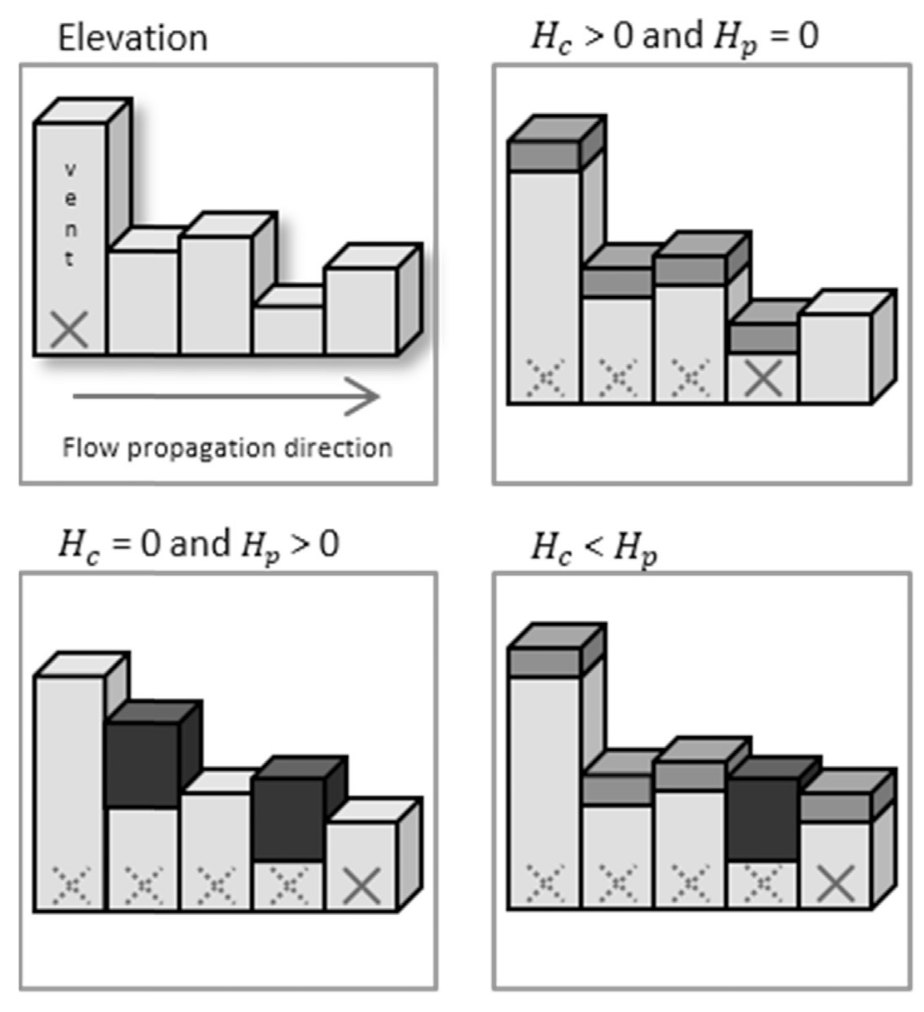
\includegraphics[width=1\textwidth]{img/qlavha_pixels.png}
%       \end{column}

%     \end{columns}
%  \end{frame}



% \begin{frame}[standout]
%   \alert{Exercise 2:} Probabilistic lava flow inundation hazard assessment for La Palma
% \end{frame}

% \begin{frame}[t]{Exercise 2: Probabilistic lava flow inundation hazard assessment}
%   \textbf{Aims:}
%   \begin{itemize}
%     \item Perform a probabilistic hazard assessment for lava flow inundation for La Palma
%     \item Contrast results when using \alert{point} vs \alert{surface} source
%   \end{itemize}
  
%   \only<2>{
%     \vspace*{1em}\textbf{Workflow:}
%     \begin{itemize}
%       \item Make sure you have installed \textbf{Q-LavHA}
%       \item Go through the \alert{Q-LavHA} exercise on http://cerg-c.github.io
%     \end{itemize}
%   }

%   \only<3>{
%     \vspace*{1em}\textbf{Don't forget:}
%     \begin{itemize}
%       \item To answer questions!
%     \end{itemize}
%   }
% \end{frame}


% \begin{frame}[standout]
%   \usebeamercolor[mWhite]{normal text}
%   Questions?\vspace*{.3cm}\\
%   \footnotesize 
\includegraphics[height=.2cm]{iconMail.pdf} \textmd{     sebastien.biasse@unige.ch}\\
%   \footnotesize 
\includegraphics[height=.25cm]{iconGit.pdf} \textmd{     e5k / http://e5k.github.io }
% \end{frame}


\end{document}







